\clearpage
\section{قوالب DOCX}
\label{sec:builder-feature-docx-templates}

قالب DOCX ملف Word عادي تكتب فيه النص الثابت، وتضع مكان البيانات المتغيرة وسوماً بين قوسين مزدوجين، مثل اسم الموظف أو رقم الطلب. وعندما يضغط المستخدم زر الإجراء في السجل، يملأ كيان الوسوم من بيانات السجل وينزّل المستند بصيغة Word أو PDF. وبذلك تُنشئ العقود والخطابات بنص موحّد دون نسخ يدوي. وتعرض هذه الصفحة قائمة القوالب وطريقة إنشاء قالب جديد، أما كتابة الوسوم والعمل داخل القالب فلكل منهما صفحة تالية.

\textbf{المسار ومن يستخدمه:} «ادوات البناء» ← «الأساسية» ← «قوالب DOCX». يديرها من يملك إدارة أدوات البناء، أما المستخدمون فيستعملونها من زر في السجل.

\begin{rcnote}[مثال: شركة الأفق]
يكتب مسؤول النظام خطاب تأكيد الزيارة في Word، ويضع وسماً لرقم الطلب وآخر لموعد الزيارة، ثم يرفعه قالباً ويربطه بزر في «طلبات الزيارة». ويرفع الخطاب من ① ويختبره بعد فتحه من ③.
\end{rcnote}

\begin{figure}[H]
\centering
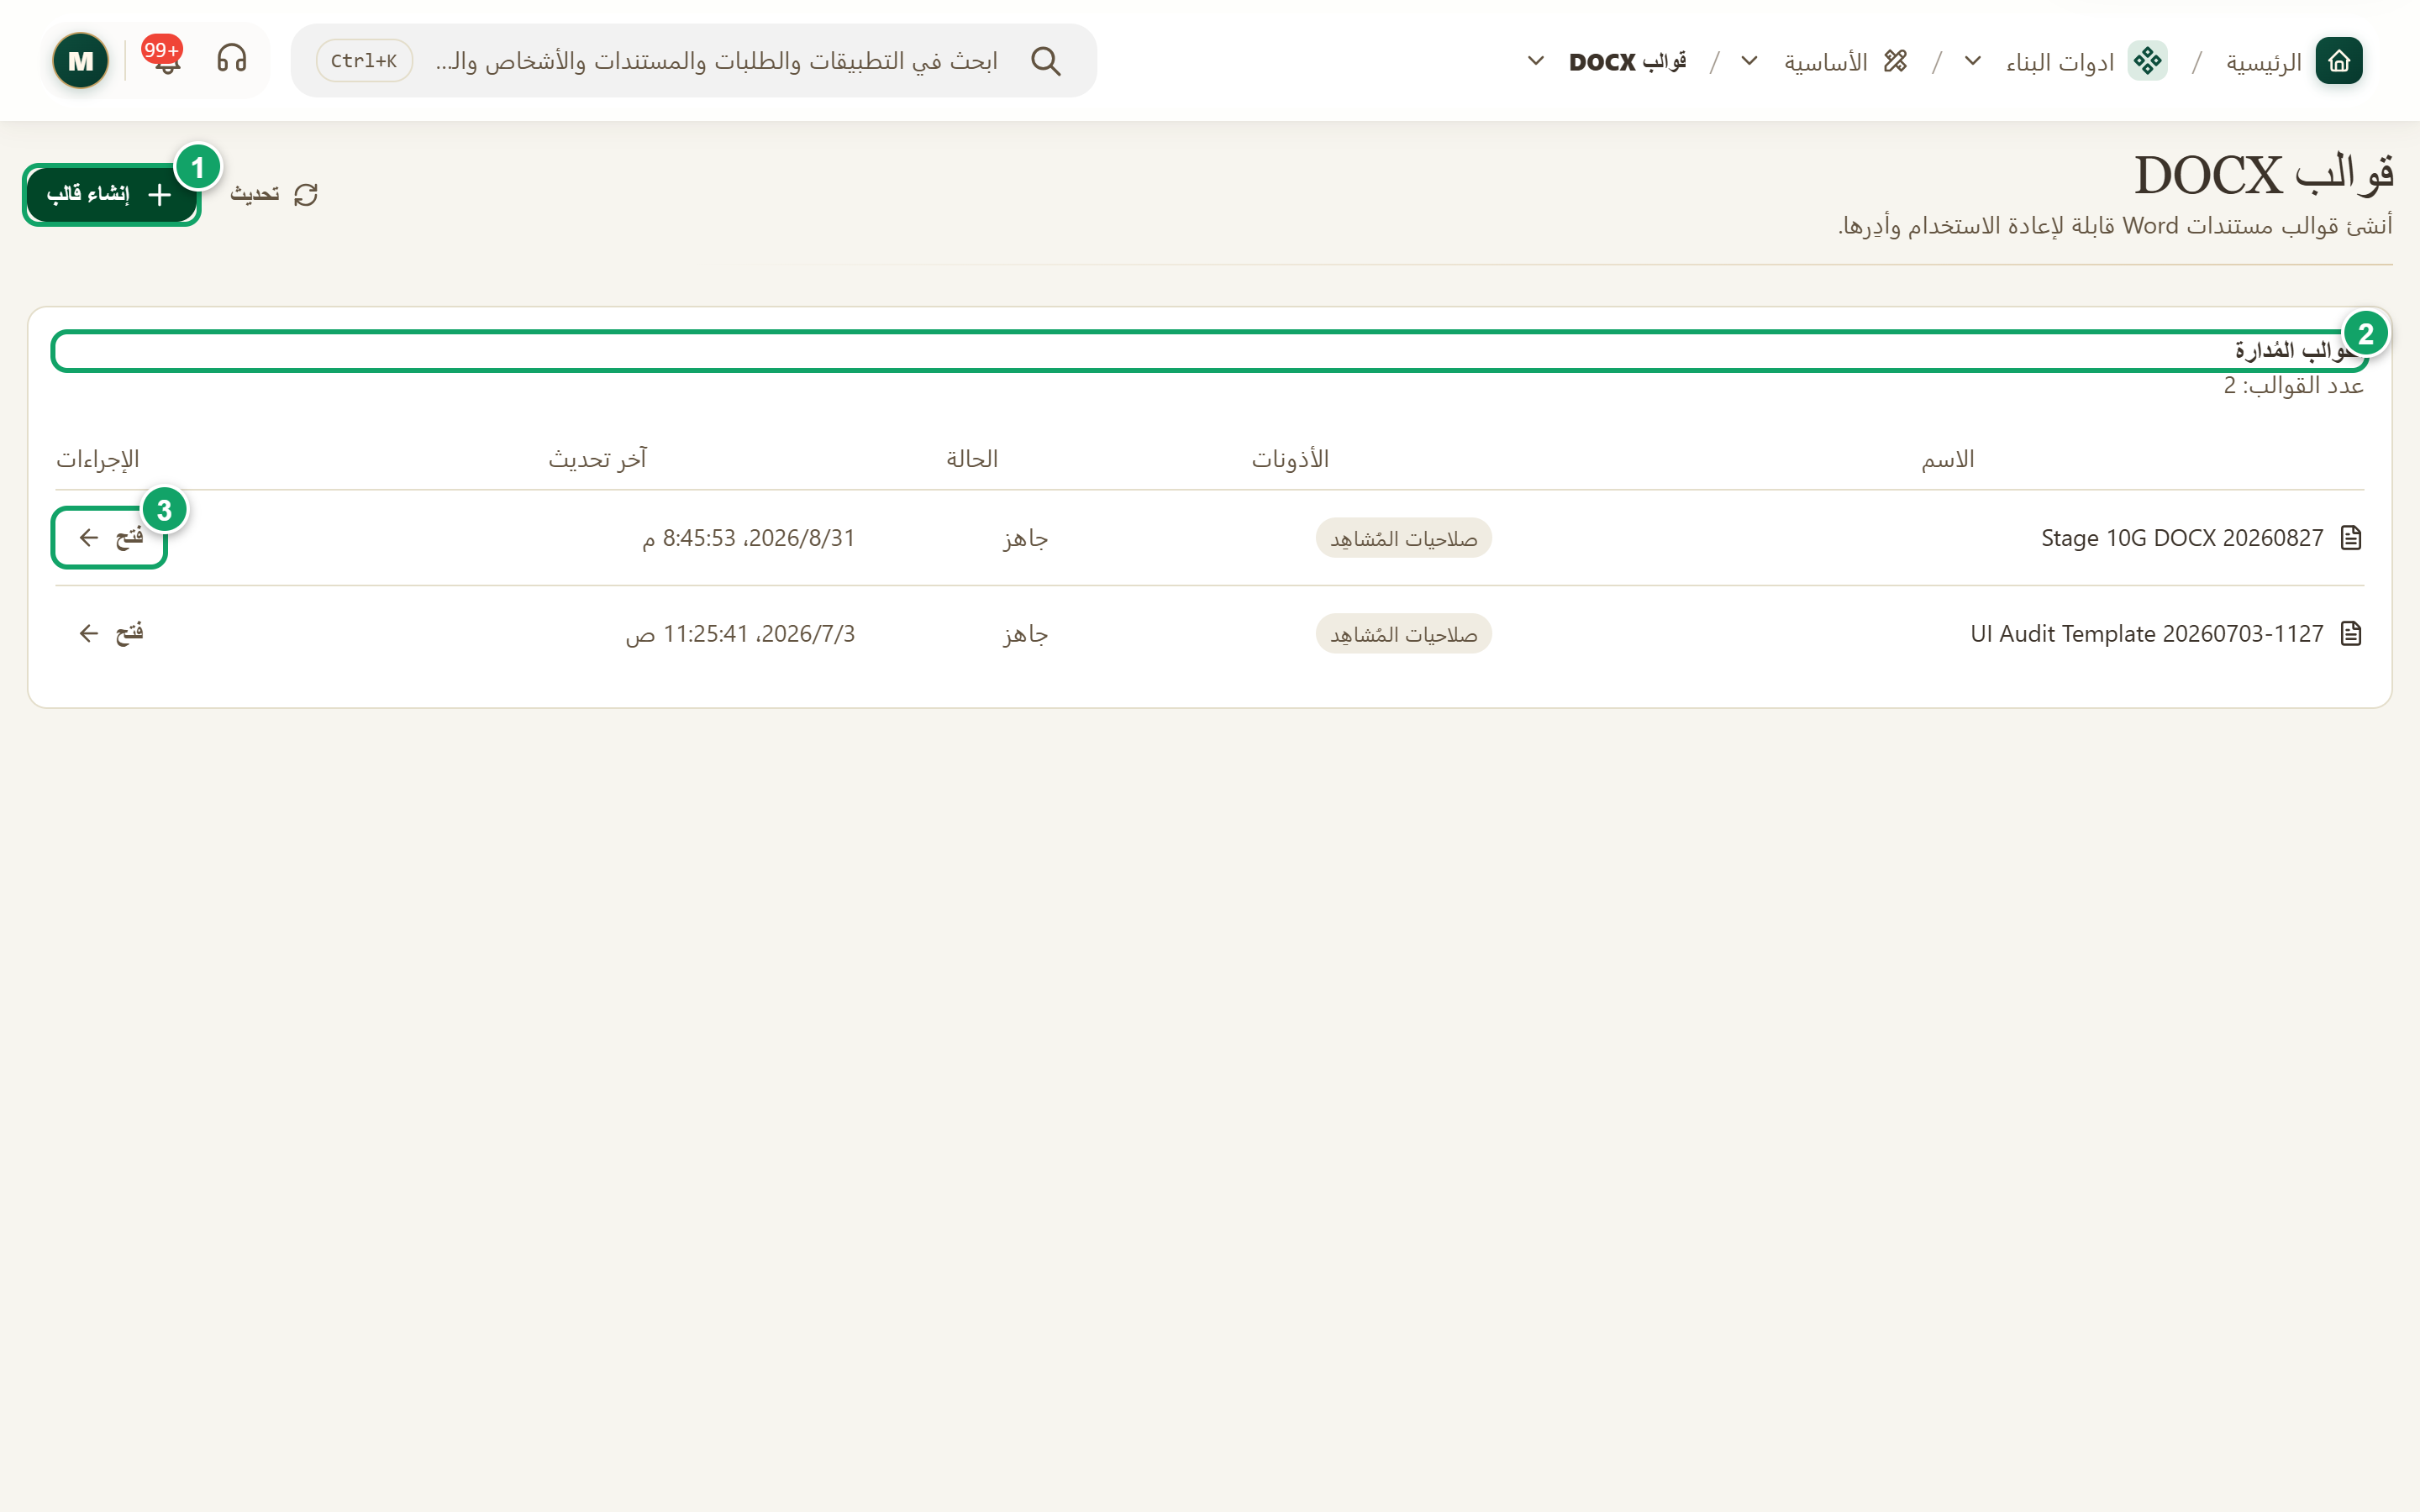
\includegraphics[width=0.95\linewidth,height=0.72\textheight,keepaspectratio]{figures/screens/ch06-docx-ar.png}
\caption{صفحة «قوالب DOCX»}
\label{fig:builder-docx-templates-screen}
\shotnote{تعرض الصفحة القوالب المُدارة وأذوناتها وحالاتها، وهي هنا قوالب اختبار. ① «إنشاء قالب»: يرفع ملف Word جديداً. ② «القوالب المُدارة»: القائمة مع حالة كل قالب. ③ «فتح»: يفتح القالب للإعدادات والإصدارات والاختبار.}
\end{figure}


\begin{table}[H]
\centering
\caption{ما الذي تجده هنا؟}
\label{tab:builder-docx-data}
\begin{tabularx}{\linewidth}{R{3.6cm} Y}
\rcHeaderRow
\thh{الجزء} & \thh{المحتوى والإجراء}\\
القوالب المُدارة & قائمة القوالب مع «الأذونات» و«الحالة»: «جاهز» عندما يوجد إصدار حالي، أو «يحتاج إلى مستند Word».\\
إنشاء قالب & ترفع «مستند Word» بصيغة \en{.docx} وحدها، وتكتب «اسم القالب» و«الوصف (اختياري)».\\
اسم الملف عند التنزيل & يقع في «الإعدادات الافتراضية المتقدمة»، ويُكتب تعبيراً يبني الاسم من بيانات السجل، مثل رقم الطلب. وإذا بقي فارغاً أو تعذّر حسابه، فيُستخدم اسم الملف المرفوع.\\
أذونات المستند & «صلاحيات المُشاهِد»، وهي الموصى بها، تعرض فقط ما يستطيع من ينزّل الملف رؤيته. أما «صلاحيات المسؤول» فقد تضع في المستند بيانات لا يراها.\\
إنشاء بمساعدة الذكاء الاصطناعي & زر يظهر عندما يكون «الذكاء الاصطناعي في أدوات البناء» مفعّلاً، فيبدأ القالب بمساعد يقترح مسودة تراجعها قبل حفظها.\\
\end{tabularx}
\end{table}

\begin{figure}[H]
\centering
\begin{tikzpicture}[node distance=0.5cm]
\node[stepBox] (a) {\RL{ملف Word بوسوم}};
\node[stepBox,below=of a] (b) {\RL{إنشاء قالب واختباره}};
\node[stepBox,below=of b] (c) {\RL{إجراء «قالب DOCX» في السجل}};
\node[stepBox,below=of c] (d) {\RL{المستخدم يضغط الزر}};
\draw[flowsTo] (a) -- (b);
\draw[flowsTo] (b) -- (c);
\draw[flowsTo] (c) -- (d);
\end{tikzpicture}
\rclegend
\caption{من ملف Word إلى مستند لكل سجل}
\label{fig:builder-docx-flow}
\shotnote{يبيّن المخطط أن القالب لا يرتبط بنوع سجلات بنفسه، بل يصل إلى المستخدم عبر إجراء من نوع «قالب DOCX» تضيفه في «الإجراءات والأتمتة». لذلك يأتي الاختبار على سجل حقيقي قبل الربط، لأن التحقق عند الرفع لا يكشف كل خطأ في موضع الوسوم.}
\end{figure}

\subsection{خطوات العمل والتحقق}
\begin{enumerate}
\item اكتب المستند في Word، وضع الوسوم بمفاتيح الحقول الفعلية، واجعل وسوم الشرط والتكرار في فقرة مستقلة.
\item افتح «قوالب DOCX» واضغط «إنشاء قالب»، ثم ارفع الملف واكتب الاسم واضغط «إنشاء قالب».
\item افتح «اختبار وتحميل»، واختر سجلاً، ثم «إنشاء وتنزيل» وراجع المستند.
\item أضف في نوع السجلات إجراءً من نوع «قالب DOCX» واختر القالب في «اختر القالب»، ثم انشر.
\end{enumerate}

\textbf{تحقق ومعالجة المشكلة:} يجب أن تظهر حالة القالب «جاهز»، وأن ينزّل زر الإجراء مستنداً ممتلئاً ببيانات السجل. فإذا ظهر «هذا المستند يحتاج إلى مراجعة» عند الرفع، فصحّح الوسوم المذكورة وأعد الرفع. وإذا ظهرت قيمة فارغة، فتأكد من أنك استخدمت مفتاح الحقل لا تسميته.

\clearpage
\section{وسوم قوالب DOCX والتكرار}
\label{sec:builder-feature-docx-tags}

الوسم نص بين قوسين مزدوجين تكتبه في ملف Word حيث يجب أن تظهر قيمة من السجل. ويقرأ كيان الوسوم عند إنشاء المستند ويستبدل بها البيانات، في متن المستند وفي رأس الصفحة وتذييلها والحواشي والتعليقات. وللوسوم ثلاثة أنواع: وسم قيمة يوضع داخل السطر مع نص آخر، ووسوم تحكم للشرط والتكرار تشغل فقرة كاملة أو صفاً كاملاً من جدول، ووسوم إضافية تُدرج صورة أو رابطاً أو رمز QR أو فاصل صفحة.

\textbf{المسار ومن يستخدمه:} تُكتب الوسوم في Word قبل رفع الملف من «ادوات البناء» ← «الأساسية» ← «قوالب DOCX». يكتبها من يدير القوالب، ويستعمل فيها مفاتيح الحقول كما تظهر في نوع السجلات.

\begin{rcnote}[مثال: شركة الأفق]
يكتب مسؤول النظام في خطاب تأكيد الزيارة سطر «موعد الزيارة:» ثم الوسم \en{\{\{ \$record.visit\_date \}\}}. ويضع حول هذا السطر فقرة شرط مستقلة، فإن لم يُحدَّد الموعد بعد ظهرت بدلاً منه جملة «سيُرسل الموعد بعد المراجعة».
\end{rcnote}

\begin{table}[H]
\centering
\caption{الوسوم وأماكنها في Word}
\label{tab:builder-docx-tags}
\begin{tabularx}{\linewidth}{R{3.6cm} Y}
\rcHeaderRow
\thh{الوسم} & \thh{ماذا يفعل؟ وأين يوضع؟}\\
\en{\{\{ \$record.field\_key \}\}} & يضع قيمة حقل بمفتاحه لا بتسميته، ويمكن أن يشارك فقرة فيها نص آخر. والقيمة الفارغة تُطبع نصاً فارغاً.\\
\en{\{\{\#if ...\}\}} و\en{\{\{else\}\}} و\en{\{\{/if\}\}} & تُظهر الفقرات التي بينها عندما يتحقق الشرط، وإلا تُظهر ما بعد \en{else}. وكل وسم منها وحده في فقرته أو صفه.\\
\en{\{\{\#each list as item\}\}} و\en{\{\{/each\}\}} & تكرر الفقرات أو صفوف الجدول التي بينها لكل عنصر. وداخلها \en{\$index} الذي يبدأ من الصفر، و\en{\$first} و\en{\$last}.\\
\en{\{\{@image ... width=120\}\}} & يُدرج صورة PNG أو JPEG أو WebP حتى 10 ميغابايت، ويُضاف \en{optional=true} حين يجوز غيابها.\\
\en{\{\{@link url label\}\}} & يُدرج رابطاً يبدأ بـ \en{http} أو \en{https} أو \en{mailto} فقط.\\
\en{\{\{@qr ... width=120\}\}} & يُنشئ رمز QR من قيمة غير فارغة، مثل رقم الطلب.\\
\en{\{\{@pageBreak\}\}} & يبدأ صفحة جديدة.\\
\en{\{\{> ...\}\}} & يُدرج متن قالب آخر، مثل بند ثابت، ويوضع وحده في فقرته. ويُسمح بخمسة مستويات إدراج متداخلة.\\
\end{tabularx}
\end{table}

\begin{table}[H]
\centering
\caption{البيانات التي يقرأ منها القالب}
\label{tab:builder-docx-tags-context}
\begin{tabularx}{\linewidth}{R{3.6cm} Y}
\rcHeaderRow
\thh{الجذر} & \thh{ما يحتويه}\\
\en{\$record} & حقول السجل المختار وبياناته العامة بمفاتيحها.\\
\en{\$inverseRelations} & السجلات التي تشير إلى هذا السجل، كما ضُبطت في الإجراء.\\
\en{\$organization} و\en{\$member} & المؤسسة الحالية والعضو الذي يُنشئ المستند.\\
\en{\$now} & وقت إنشاء المستند، وتنسّقه بنفسك.\\
\en{getRecords} & دالة تجلب سجلات من نوع آخر بحد أقصى 500 سجل في كل استدعاء، وتخضع لصلاحيات من ينزّل المستند ما لم يُضبط القالب على «صلاحيات المسؤول».\\
\end{tabularx}
\end{table}

\begin{rcwarn}[التحقق عند الرفع لا يضمن موضع الوسوم]
يكتشف التحقق الوسوم الفارغة أو غير المغلقة والأوامر غير المدعومة، مثل \en{@html} و\en{@chart} وإدراج XML الخام. لكنه لا يضمن أن وسم الشرط أو التكرار يشغل فقرته وحده، فقد ينجح الرفع ثم يختفي النص أو يُطبع الوسم. لذلك اختبر كل شرط وتكرار على سجل حقيقي بعد كل تعديل.
\end{rcwarn}

\begin{figure}[H]
\centering
\begin{tikzpicture}[node distance=0.5cm]
\node[stepBox] (a) {\RL{وسوم القيم داخل السطر}};
\node[stepBox,below=of a] (b) {\RL{وسوم الشرط والتكرار}\\\RL{في فقرات مستقلة}};
\node[stepBox,below=of b] (c) {\RL{الرفع والتحقق}};
\node[stepBox,below=of c] (d) {\RL{الاختبار على سجل حقيقي}};
\draw[flowsTo] (a) -- (b);
\draw[flowsTo] (b) -- (c);
\draw[flowsTo] (c) -- (d);
\end{tikzpicture}
\rclegend
\caption{ترتيب كتابة الوسوم واختبارها}
\label{fig:builder-docx-tags-flow}
\shotnote{يفصل المخطط بين وسوم القيم التي تعيش داخل الجملة ووسوم التحكم التي تحتاج إلى فقرة أو صف كامل، لأن الخلط بينهما أكثر أسباب الأخطاء شيوعاً. وينتهي بالاختبار على سجل حقيقي، فهو وحده يثبت أن الشرط والتكرار يعملان كما تريد.}
\end{figure}

\subsection{خطوات العمل والتحقق}
\begin{enumerate}
\item اكتب في Word كل وسم قيمة بمفتاح الحقل، مثل \en{\{\{ \$record.field\_key \}\}}، داخل الجملة التي يخصها.
\item ضع وسم بداية الشرط أو التكرار في فقرة مستقلة، ثم الفقرات أو صف الجدول الذي يتكرر، ثم وسم النهاية في فقرة مستقلة.
\item أضف الصور والروابط ورموز QR بالوسوم المخصصة لها، واكتب خياراتها دون مسافات داخل القيم.
\item ارفع الملف، فإذا ظهر «هذا المستند يحتاج إلى مراجعة» فصحّح المشكلات المذكورة وأعد الرفع.
\item اختبر القالب على سجل ممتلئ وآخر تنقصه بعض القيم، وعلى قائمة فارغة وأخرى فيها عدة عناصر.
\end{enumerate}

\textbf{تحقق ومعالجة المشكلة:} يجب أن تُستبدل كل الوسوم بقيم، وأن تختفي وسوم التحكم من الملف الناتج. فإذا طُبع وسم شرط أو اختفى نص حوله، فانقل الوسم إلى فقرة مستقلة. وإذا لم يتكرر أي صف، فتأكد من أن التعبير يُرجع قائمة، ومن أن الاسم المستعار بعد \en{as} مكتوب كما تستخدمه داخل الحلقة.

\clearpage
\section{مساحة عمل قالب DOCX ومساعد الذكاء الاصطناعي}
\label{sec:builder-feature-docx-workspace}

عندما تضغط «فتح» بجانب قالب تنتقل إلى مساحة عمله، وفيها ثلاثة تبويبات: «الإعدادات» و«الإصدارات» و«اختبار وتحميل». وتعرض شارة في رأسها «جاهز للاستخدام» إذا كان للقالب إصدار حالي، أو «يتطلب إصدار DOCX». ومن هنا تعدّل القالب وتستبدل ملفه وتجرّبه قبل أن يصل إلى المستخدمين. وإذا كان «الذكاء الاصطناعي في أدوات البناء» مفعّلاً، فيمكنك أن تطلب من المساعد تعديل القالب، فيقترح مسودة لا تُحفظ إلا بعد مراجعتك.

\textbf{المسار ومن يستخدمه:} «ادوات البناء» ← «الأساسية» ← «قوالب DOCX» ← «فتح». يستخدمها من يدير القوالب كلما عدّل نص المستند أو أراد تجربته.

\begin{rcnote}[مثال: شركة الأفق]
يختبر مسؤول النظام خطاب تأكيد الزيارة على الطلب HZN-VR-0001 بصيغة PDF. ثم يفتح «الإصدارات» ويطلب من المساعد أن يجعل التحية أكثر رسمية، ويراجع المسودة قبل اعتمادها. فيختبر من ①، ثم يفتح ② ويبدأ المساعد من ④.
\end{rcnote}

\begin{figure}[H]
\centering
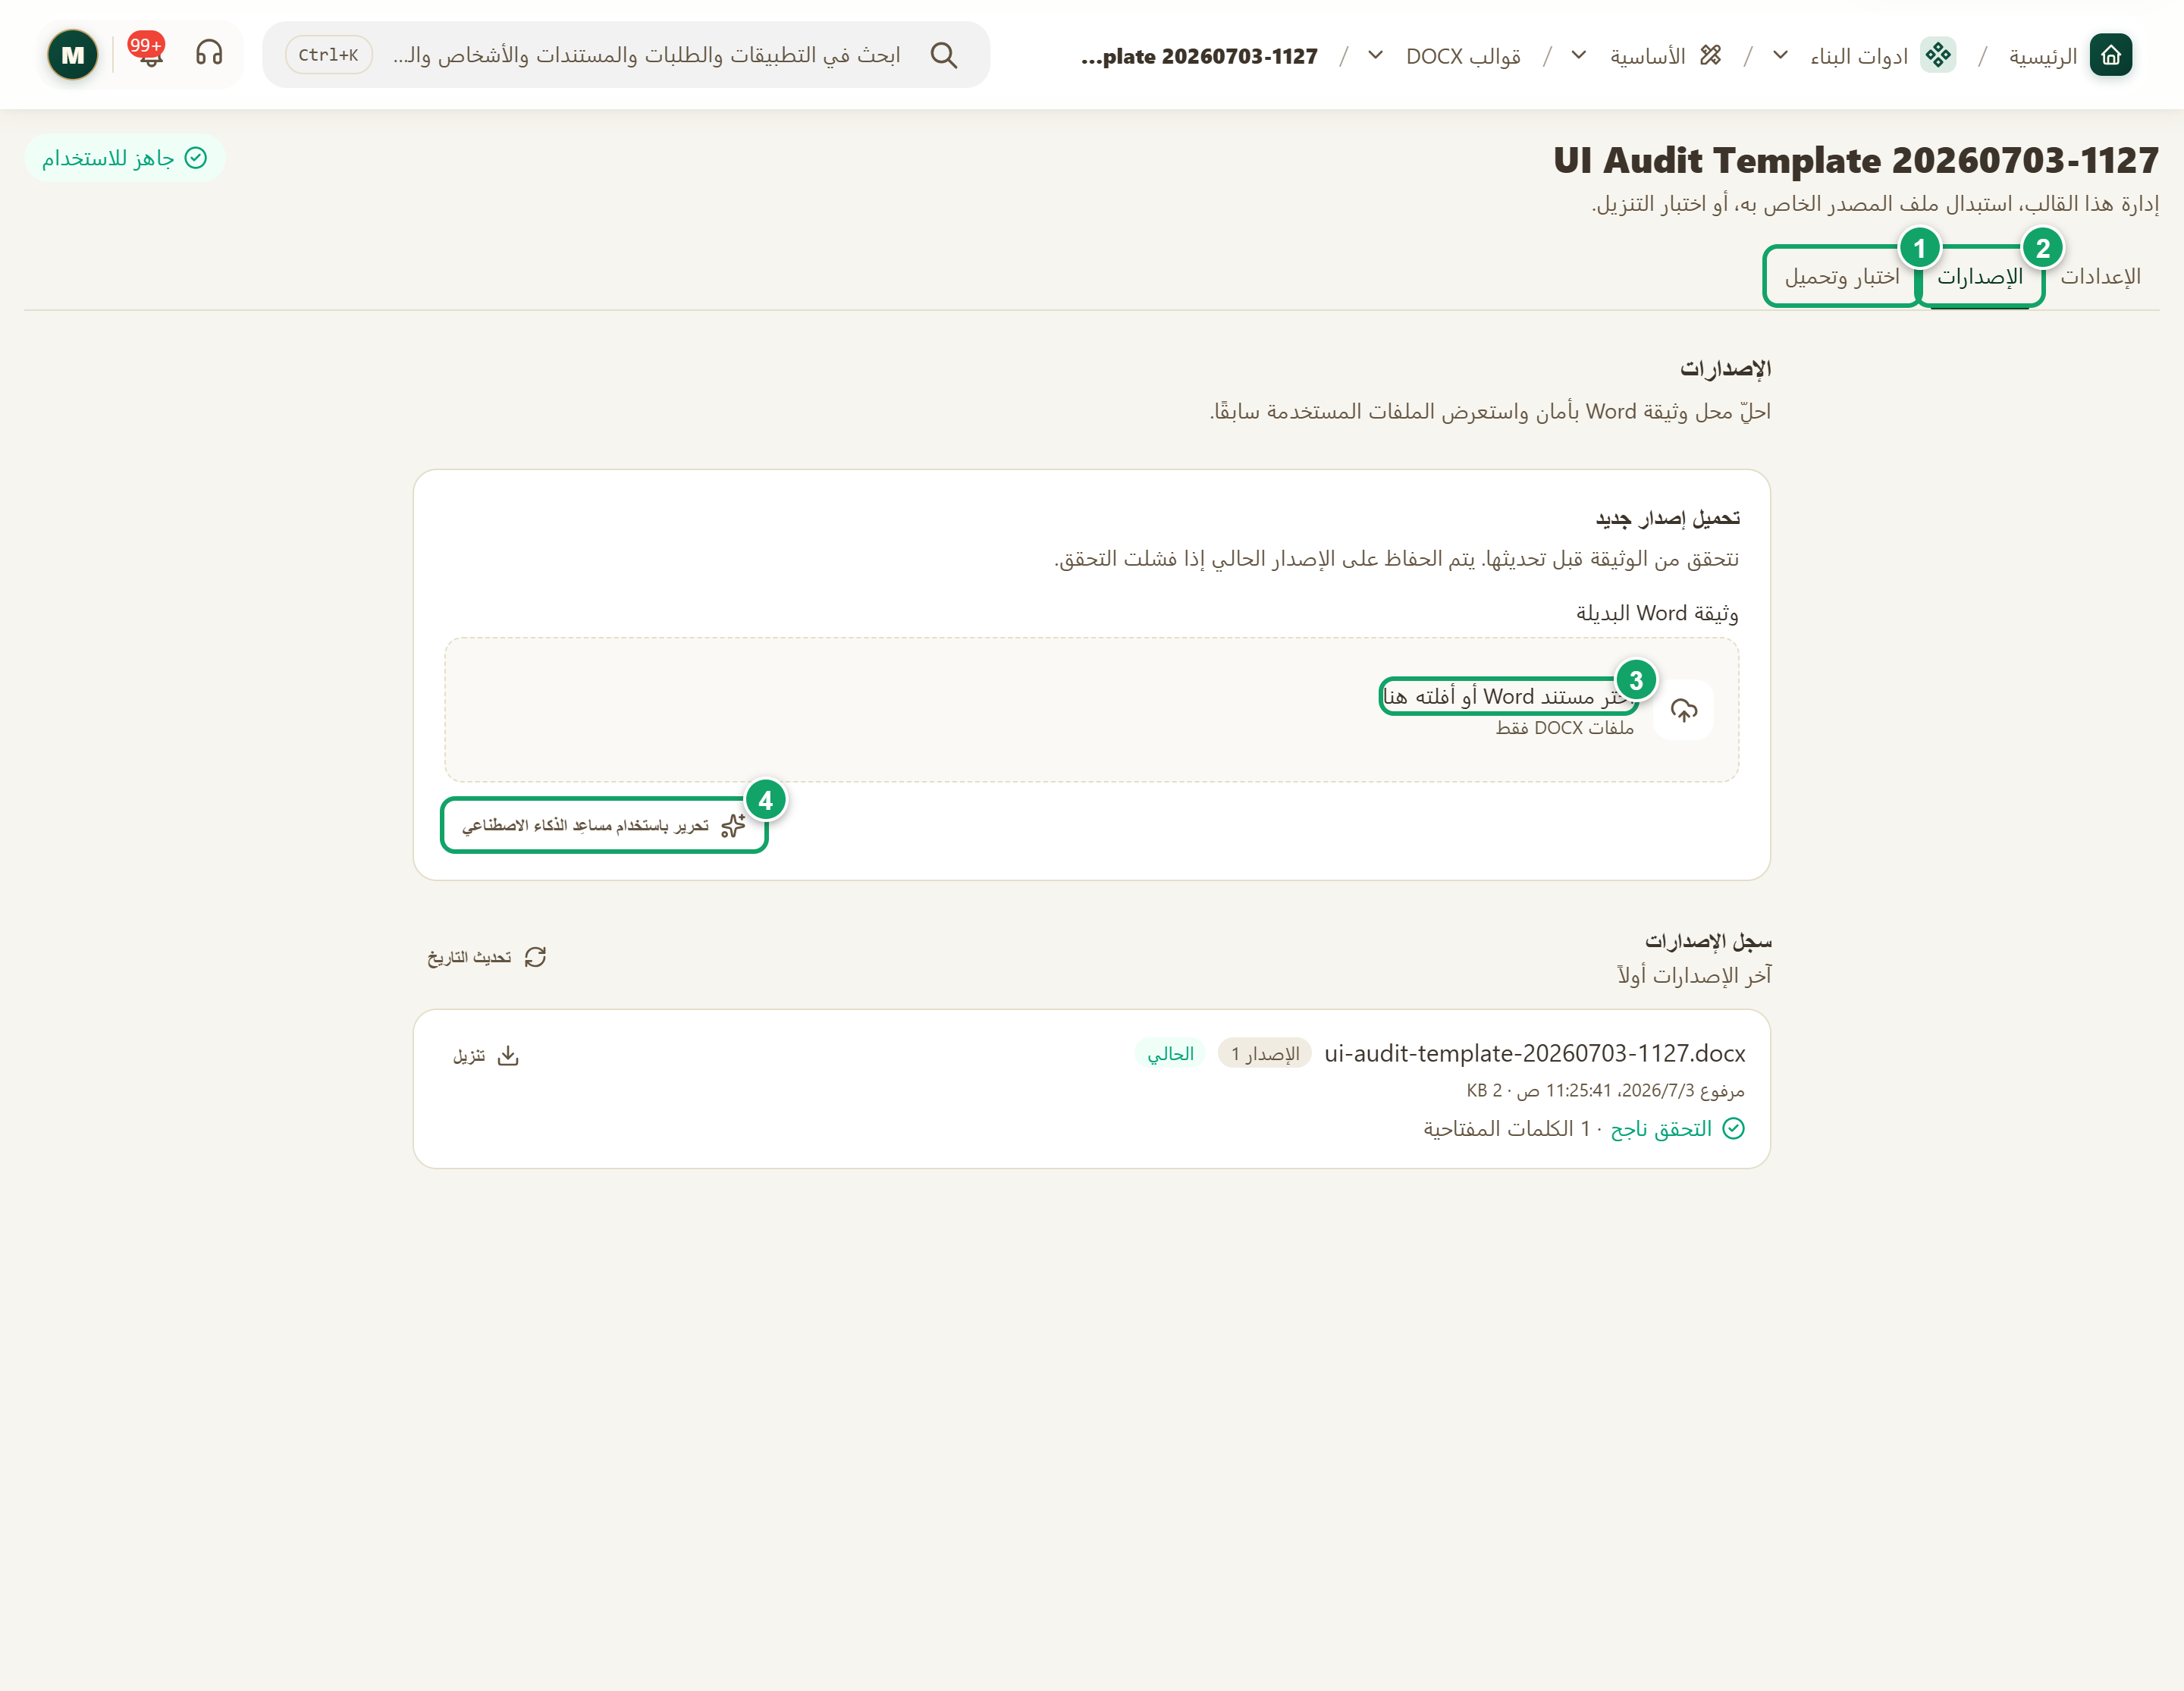
\includegraphics[width=0.95\linewidth,height=0.72\textheight,keepaspectratio]{figures/screens/ch06-docx-workspace-ar.png}
\caption{تبويب «الإصدارات» في مساحة عمل قالب DOCX}
\label{fig:builder-docx-workspace-screen}
\shotnote{تعرض الصورة قالب DOCX اختبارياً في test2 مفتوحاً على تبويب «الإصدارات»، وتحته «سجل الإصدارات» الذي يبيّن الإصدار الحالي ونتيجة التحقق منه. وتجمع هذه الشاشة طريقتي إنشاء إصدار جديد: رفع ملف بديل، أو طلب مسودة من المساعد، ولذلك يسبقهما الاختبار. ① «اختبار وتحميل»: تجرّب فيه القالب على سجل قبل أي تعديل. ② «الإصدارات»: التبويب المعروض. ③ «اختر مستند Word أو أفلته هنا»: تختار منه ملف الإصدار البديل. ④ «تحرير باستخدام مساعِد الذكاء الاصطناعي»: يفتح صفحة المساعد لاختيار السياق وكتابة الطلب.}
\end{figure}

\begin{table}[H]
\centering
\caption{تبويبات مساحة العمل}
\label{tab:builder-docx-workspace-tabs}
\begin{tabularx}{\linewidth}{R{3.6cm} Y}
\rcHeaderRow
\thh{التبويب} & \thh{المحتوى والإجراء}\\
الإعدادات & «اسم القالب» و«الوصف (اختياري)» واسم الملف عند التنزيل و«أذونات المستند»، ثم «حفظ التغييرات».\\
الإصدارات & تختار ملف Word بديلاً وتضغط زر التحقق والرفع، فيتحقق كيان من الملف قبل أن يجعله الإصدار الحالي. ويعرض «سجل الإصدارات» الإصدارات من الأحدث، مع علامة «الحالي» ونتيجة التحقق وزر «تنزيل».\\
اختبار وتحميل & تختار بيانات الاختبار: «استخدم سجلاً» أو «لصق JSON — متقدم»، ثم الصيغة Word أو PDF. وتغيّر «خيارات متقدمة» اسم الملف والأذونات لهذا التنزيل فقط، ثم تضغط «إنشاء وتنزيل».\\
\end{tabularx}
\end{table}

\begin{table}[H]
\centering
\caption{مساعد DOCX بالذكاء الاصطناعي}
\label{tab:builder-docx-workspace-ai}
\begin{tabularx}{\linewidth}{R{3.6cm} Y}
\rcHeaderRow
\thh{المرحلة} & \thh{ما يحدث فيها}\\
البدء & من «إنشاء بمساعدة الذكاء الاصطناعي» عند إنشاء قالب، أو «تحرير باستخدام مساعِد الذكاء الاصطناعي» في «الإصدارات» لتعديل الإصدار الحالي.\\
السياق & تختار «استخدم سياق الكيان» مع سجل اختياري، فإن لم تختر سجلاً استُخدمت بيانات عينة. أو تختار «JSON يدوي» في حدود 256 كيلوبايت.\\
الموافقة على الإرسال & تؤكد أن نص المستند والسياق وتعليماتك سترسل إلى مزود الذكاء الاصطناعي الذي ضبطته المؤسسة. أما ملف Word نفسه فلا يُرسل.\\
المراجعة & كل طلب ينشئ مراجعة مرقّمة، فتقرأ «ملخص التغيير» و«رموز القالب»، وتعرض معاينة أو تضغط «تنزيل DOCX». ويجب أن تحل كل سؤال في «أسئلة لحلها» قبل الاعتماد.\\
الاعتماد أو الحذف & زر الموافقة والحفظ ينشئ إصداراً جديداً دون تغيير إعدادات القالب أو الإجراءات المرتبطة به، و«حذف المسودة» يلغيها. وتنتهي المسودة بعد 24 ساعة دون نشاط، وبعد سبعة أيام على الأكثر.\\
\end{tabularx}
\end{table}

\begin{rcwarn}[الإصدار الجديد يعمل فوراً]
تستخدم أزرار الإجراءات في السجلات الإصدار الحالي دائماً، لذلك يصل أي إصدار ترفعه أو تعتمده إلى المستخدمين مباشرة. فاختبر الملف على سجل حقيقي قبل رفعه، واحتفظ بنسخة من الملف المعتمد خارج كيان.
\end{rcwarn}

\begin{figure}[H]
\centering
\begin{tikzpicture}[node distance=0.5cm]
\node[stepBox] (a) {\RL{فتح القالب}};
\node[stepBox,below=of a] (b) {\RL{اختبار وتحميل على سجل}};
\node[stepBox,below=of b] (c) {\RL{إصدار جديد: رفع ملف}\\\RL{أو مسودة من المساعد}};
\node[stepBox,below=of c] (d) {\RL{المراجعة والاختبار}};
\node[stepBox,below=of d] (e) {\RL{يصبح الإصدار الحالي}};
\draw[flowsTo] (a) -- (b);
\draw[flowsTo] (b) -- (c);
\draw[flowsTo] (c) -- (d);
\draw[flowsTo] (d) -- (e);
\end{tikzpicture}
\rclegend
\caption{تعديل قالب DOCX بأمان}
\label{fig:builder-docx-workspace-flow}
\shotnote{يجمع المخطط طريقتي إنشاء إصدار جديد: رفع ملف بديل، أو اعتماد مسودة اقترحها المساعد. وفي الطريقتين تأتي المراجعة قبل أن يصبح الإصدار حالياً، لأن الإجراءات في السجلات تستخدمه منذ تلك اللحظة.}
\end{figure}

\subsection{خطوات العمل والتحقق}
\begin{enumerate}
\item افتح القالب، ثم افتح «اختبار وتحميل» واختر «استخدم سجلاً» وحدد سجلاً حقيقياً.
\item اختر الصيغة، واضغط «إنشاء وتنزيل»، وراجع الملف الناتج.
\item لتعديل النص يدوياً، افتح «الإصدارات» واختر ملف Word البديل، ثم اضغط زر التحقق والرفع.
\item لتعديله بالمساعد، اضغط «تحرير باستخدام مساعِد الذكاء الاصطناعي»، واختر السياق، واكتب طلباً واحداً محدداً في «تعليمات»، ثم أكّد موافقتك على الإرسال واضغط «ابدأ مساعداً ذكياً». أما الطلبات اللاحقة فترسلها بزر «إنشاء مسودة».
\item راجع «ملخص التغيير» والمعاينة، وحل الأسئلة المفتوحة، ثم اضغط زر الموافقة والحفظ.
\end{enumerate}

\textbf{تحقق ومعالجة المشكلة:} يجب أن تظهر رسالة «إصدار جديد للقالب جاهز للاستخدام.» وأن يحمل الإصدار الجديد علامة «الحالي» في «سجل الإصدارات». فإذا ظهر «لم يتم تحميل هذا المستند»، فاضغط «عرض المشكلات» وصحّح الملف، ويبقى الإصدار السابق نشطاً حتى ذلك الحين. وإذا لم يظهر زر المساعد، فاطلب من مسؤول المؤسسة تفعيل «الذكاء الاصطناعي في أدوات البناء».

\clearpage
\section{قوالب XLSX}
\label{sec:builder-feature-xlsx-templates}

قالب XLSX مصنف Excel فيه وسوم بالطريقة نفسها، يملؤه كيان من بيانات السجل وينزّله بصيغة Excel أو PDF. ويناسب الكشوف والتقارير الجدولية التي تتكرر صفوفها، لأن الوسوم تستطيع تكرار الصفوف والأعمدة. ويحافظ الوسم الموضوع وحده في خلية على نوع القيمة رقماً أو تاريخاً.

\textbf{المسار ومن يستخدمه:} «ادوات البناء» ← «الأساسية» ← «قوالب XLSX». يديرها من يملك إدارة أدوات البناء.

\begin{rcnote}[مثال: شركة الأفق]
يجهّز مسؤول النظام مصنف «كشف زيارات الفرع» يكرر صفاً لكل زيارة، ويربطه بزر إجراء من نوع «قالب XLSX»، فتنزّل سارة الخطيب الكشف جاهزاً بصيغة Excel. ويرفع المصنف من ①.
\end{rcnote}

\begin{figure}[H]
\centering
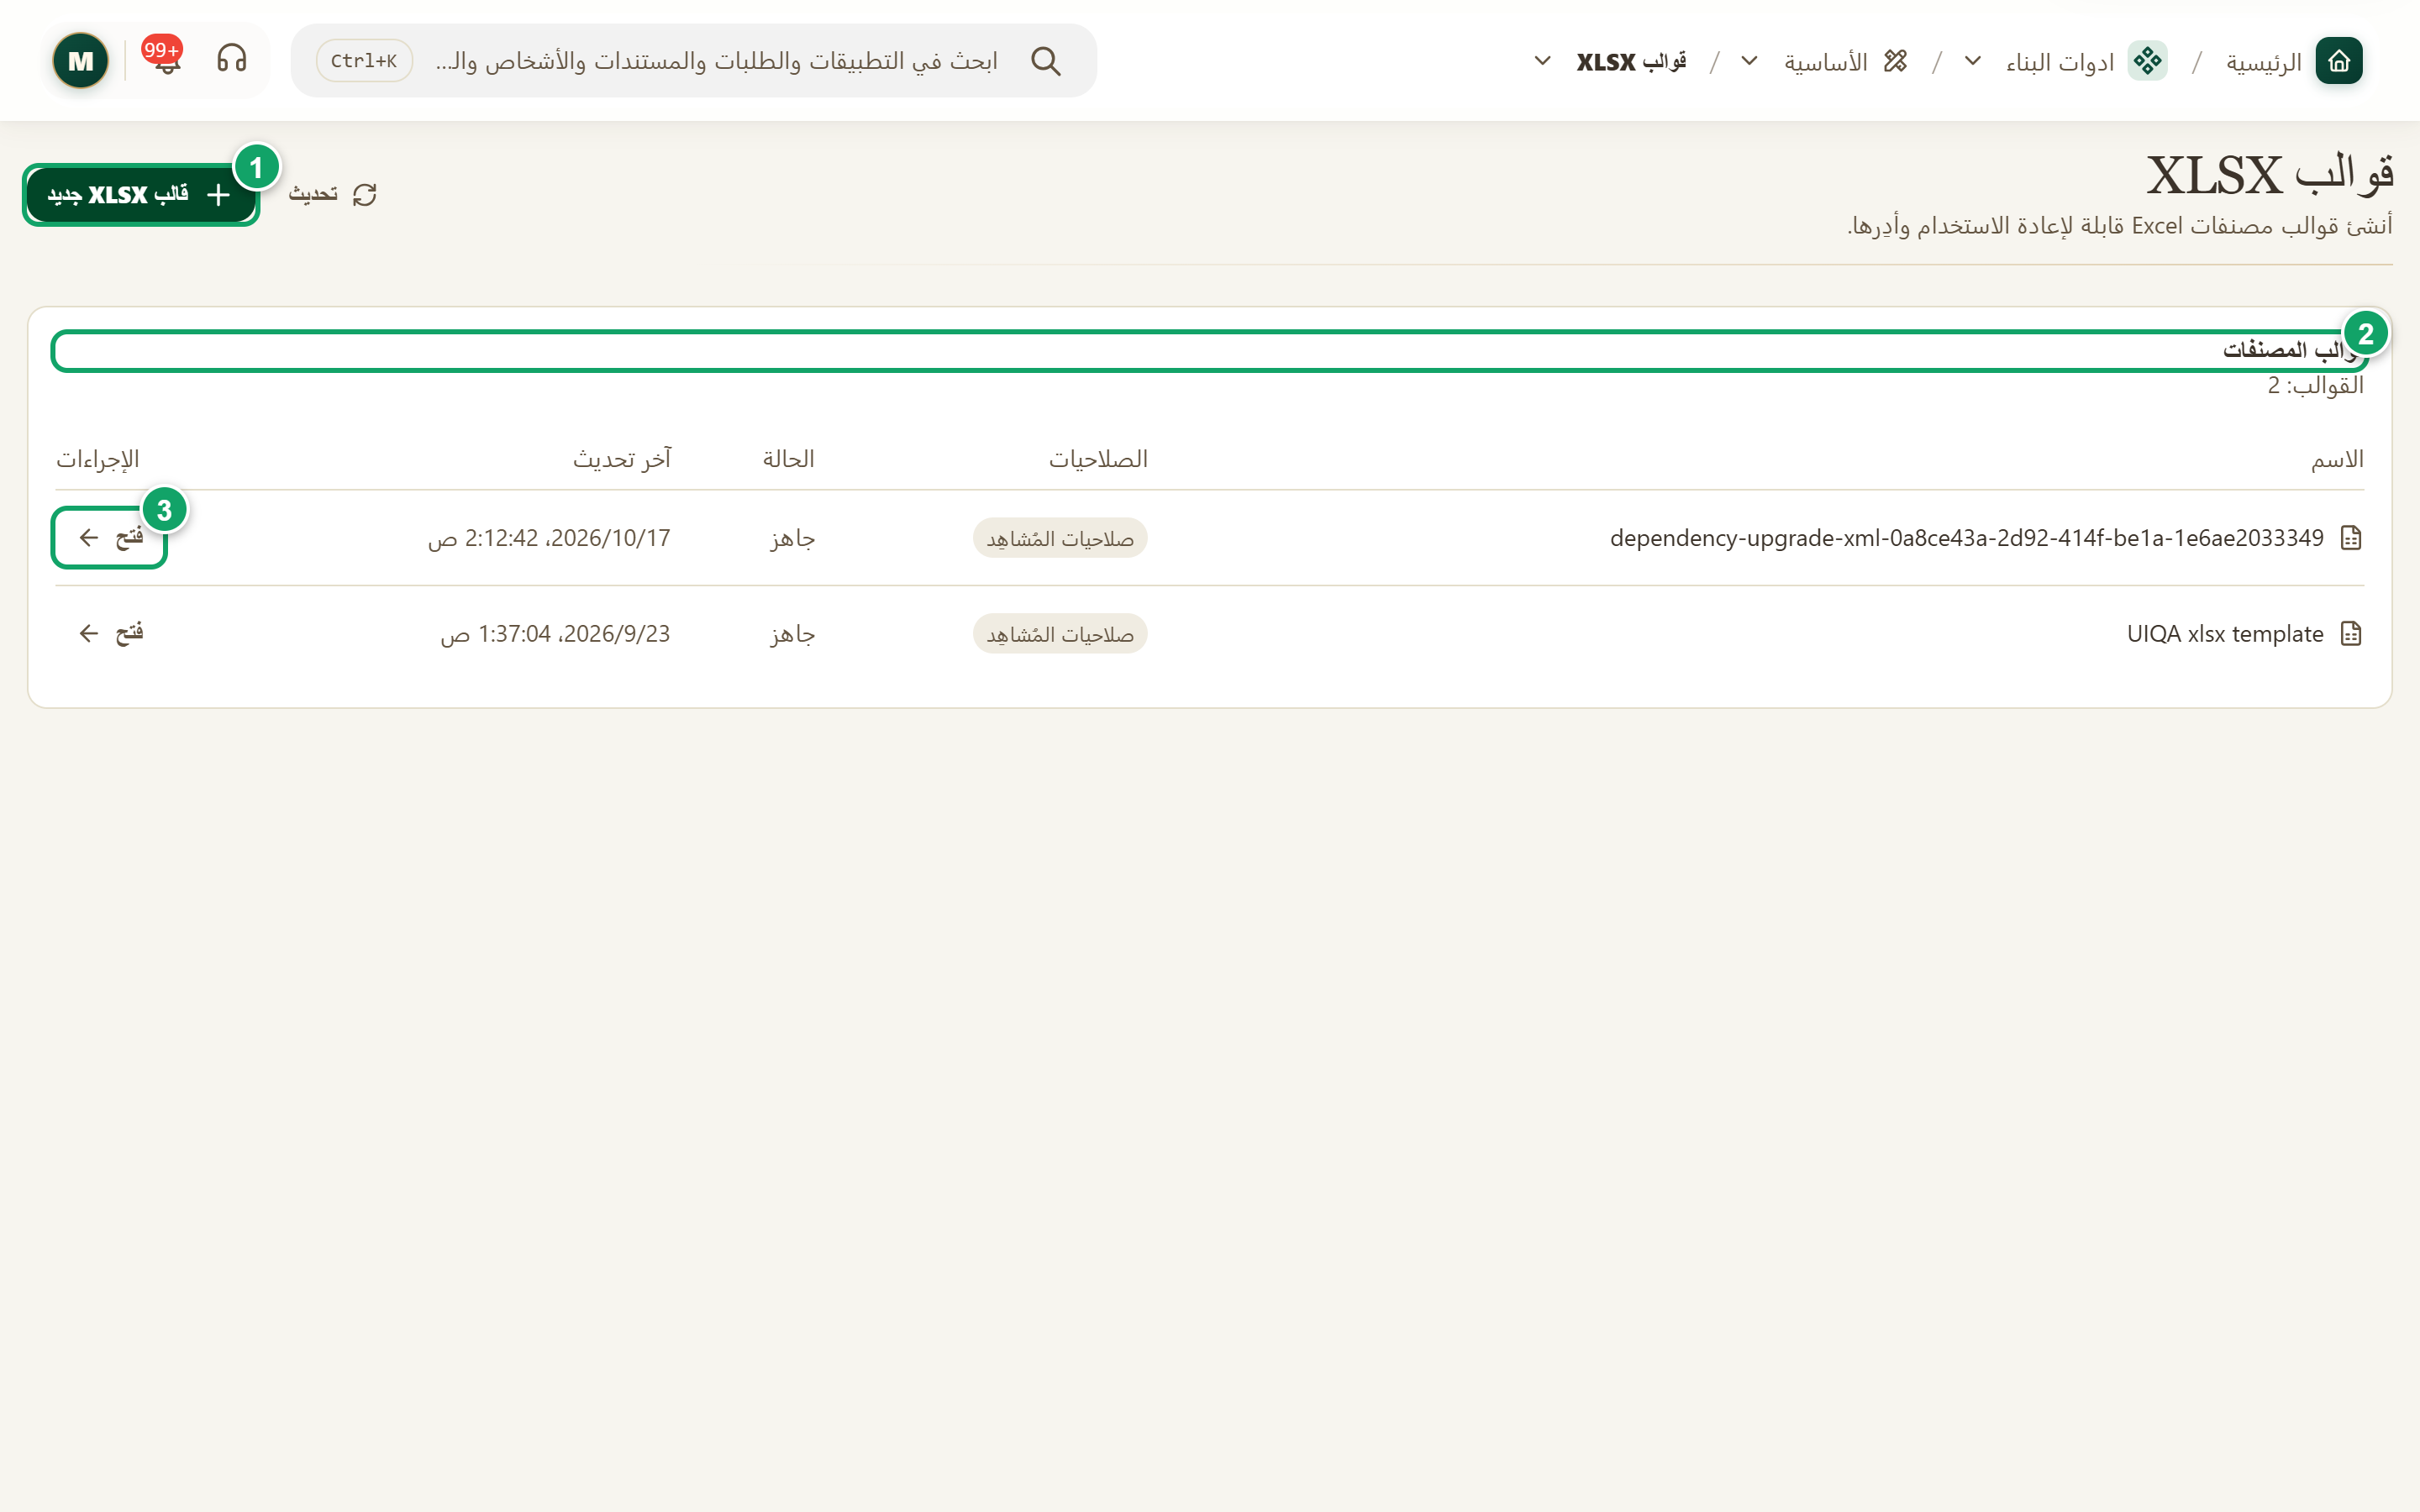
\includegraphics[width=0.95\linewidth,height=0.72\textheight,keepaspectratio]{figures/screens/ch06-xlsx-ar.png}
\caption{صفحة «قوالب XLSX»}
\label{fig:builder-xlsx-templates-screen}
\shotnote{تعرض الصفحة قوالب المصنفات وحالاتها، وهي هنا قوالب اختبار. ① «قالب XLSX جديد»: يرفع مصنف Excel. ② «قوالب المصنفات»: القائمة مع الحالة. ③ «فتح»: يفتح القالب لاختباره.}
\end{figure}


\begin{table}[H]
\centering
\caption{ما الذي تجده هنا؟}
\label{tab:builder-xlsx-data}
\begin{tabularx}{\linewidth}{R{3.6cm} Y}
\rcHeaderRow
\thh{الجزء} & \thh{المحتوى والإجراء}\\
قوالب المصنفات & قائمة القوالب وحالتها: «جاهز» أو «يحتاج إلى مصنف Excel».\\
قالب XLSX جديد & ترفع «مصنف Excel» وتكتب «اسم القالب»، ويمكنك ضبط «صيغة اسم الملف عند التنزيل» و«أذونات البيانات».\\
التحقق عند الرفع & يرفض كيان المصنفات التي فيها وحدات ماكرو أو كائنات مضمّنة أو روابط إلى مصنفات خارجية، ويعرض المشكلات تحت «هذا المصنف يحتاج إلى مراجعة».\\
الإصدارات & استبدال المصنف بإصدار جديد ومراجعة الإصدارات السابقة.\\
اختبار وتحميل & تجربة القالب ببيانات، ثم «إنشاء XLSX» أو «إنشاء PDF».\\
\end{tabularx}
\end{table}

\begin{figure}[H]
\centering
\begin{tikzpicture}[node distance=0.5cm]
\node[entity] (tpl) {\RL{قالب XLSX}};
\node[entityOpt,below right=0.7cm and 0.3cm of tpl] (xlsx) {\RL{ملف Excel}};
\node[entityOpt,below left=0.7cm and 0.3cm of tpl] (pdf) {\RL{ملف PDF}};
\draw[dependsOnOpt] (tpl.south) -- ++(0,-0.3) -| (xlsx.north);
\draw[dependsOnOpt] (tpl.south) -- ++(0,-0.3) -| (pdf.north);
\end{tikzpicture}
\rclegend
\caption{صيغتا الإخراج}
\label{fig:builder-xlsx-outputs}
\shotnote{يوضّح الشكل أن القالب الواحد يُخرج ملف Excel أو PDF، وتختار ما يُسمح به عند ربطه بالإجراء عبر «السماح بملفات PDF». فاستخدم Excel عندما يحتاج المستلم إلى معالجة الأرقام، وPDF عندما تريد نسخة ثابتة للعرض أو الأرشيف.}
\end{figure}

\subsection{خطوات العمل والتحقق}
\begin{enumerate}
\item جهّز المصنف في Excel، وضع الوسوم في الخلايا المناسبة.
\item افتح «قوالب XLSX» واضغط «قالب XLSX جديد»، ثم ارفع المصنف واكتب الاسم واضغط «إنشاء قالب».
\item جرّب القالب من «اختبار وتحميل»، ثم أضف إجراءً من نوع «قالب XLSX» في نوع السجلات واختر القالب.
\end{enumerate}

\textbf{تحقق ومعالجة المشكلة:} يجب أن تظهر حالة القالب «جاهز»، وأن يتكرر الصف لكل عنصر في الملف الناتج. فإذا ظهر رقم نصاً، فاجعل الوسم وحده في خليته. وإذا تعذّر عليك إنشاء القالب، فإدارة القوالب تحتاج إلى صلاحية إدارة أدوات البناء لا إلى مقعد كامل فقط.

\clearpage
\section{وسوم قوالب XLSX والطباعة}
\label{sec:builder-feature-xlsx-tags}

تُكتب وسوم المصنف في الخلايا العادية، والفرق الأهم عن Word هو الاتجاه: وسم \en{each} يكرر الصفوف إلى الأسفل، ووسم \en{eachCol} يكرر الأعمدة إلى الجانب. وعندما يتقاطع تكرار صفوف مع تكرار أعمدة ينتج جدول كامل، فيه صف لكل عنصر من القائمة الأولى وعمود لكل عنصر من الثانية. ويحافظ كيان على الصيغ والتنسيق والمخططات وإعدادات الطباعة الموجودة في المصنف، ويعدّل مراجعها عندما تتوسع الصفوف والأعمدة.

\textbf{المسار ومن يستخدمه:} تُكتب الوسوم في Excel قبل رفع المصنف من «ادوات البناء» ← «الأساسية» ← «قوالب XLSX». يكتبها من يدير القوالب.

\begin{rcnote}[مثال: شركة الأفق]
يضع مسؤول النظام في «كشف زيارات الفرع» تكرار صفوف لكل فرع وتكرار أعمدة لكل شهر. فيظهر في الملف الناتج صف للمقر الرئيسي في دمشق وآخر لفرع حلب، وفي كل خلية عدد زيارات الفرع في ذلك الشهر.
\end{rcnote}

\begin{table}[H]
\centering
\caption{وسوم الخلايا والتكرار}
\label{tab:builder-xlsx-tags-loops}
\begin{tabularx}{\linewidth}{R{3.6cm} Y}
\rcHeaderRow
\thh{الوسم} & \thh{ماذا يفعل؟ وأين يوضع؟}\\
\en{\{\{ \$record.field\_key \}\}} & إذا كان وحده في الخلية بقي رقماً أو قيمة منطقية أو خلية فارغة، وإذا جاء مع نص آخر صار نصاً. والنص الذي يبدأ بـ \en{=} أو \en{+} أو \en{-} أو \en{@} يبقى نصاً ولا يتحول إلى صيغة.\\
\en{\{\{\#each list as item\}\}} و\en{\{\{/each\}\}} & يكرران صفوف المتن التي بينهما. ويوضع كل منهما في صف مستقل لا يحتوي أي خلية أخرى غير فارغة.\\
\en{\{\{\#if ...\}\}} و\en{\{\{else\}\}} و\en{\{\{/if\}\}} & تختار صفوفاً حسب شرط، ويوضع كل منها في صف مستقل بالطريقة نفسها.\\
\en{\{\{\#eachCol list as item\}\}} و\en{\{\{/eachCol\}\}} & يكرران الأعمدة التي بينهما. ويوضع كل منهما في عمود مستقل لا يحتوي أي خلية أخرى غير فارغة.\\
\en{\{\{\#ifCol ...\}\}} و\en{\{\{elseCol\}\}} و\en{\{\{/ifCol\}\}} & تختار أعمدة حسب شرط، ويوضع كل منها في عمود علامة مستقل.\\
\end{tabularx}
\end{table}

\begin{table}[H]
\centering
\caption{التوجيهات والصيغ والطباعة}
\label{tab:builder-xlsx-tags-directives}
\begin{tabularx}{\linewidth}{R{3.6cm} Y}
\rcHeaderRow
\thh{العنصر} & \thh{ما يجب أن تعرفه}\\
\en{\{\{@hideRow ...\}\}} و\en{\{\{@hideColumn ...\}\}} & يخفيان الصف أو العمود الناتج عندما يكون التعبير صحيحاً.\\
\en{\{\{@link url label\}\}} & رابط آمن يبدأ بـ \en{http} أو \en{https} أو \en{mailto}.\\
\en{\{\{@image ... width=120\}\}} و\en{\{\{@qr ... width=120\}\}} & صورة أو رمز QR يشغل خلية كاملة، ويتحرك مع الصفوف والأعمدة المتوسعة.\\
الصيغ & تبقى الصيغ كما هي، وتتعدّل مراجعها مع احترام المراجع الثابتة مثل \en{\$A1} و\en{A\$1}. ولا يحسب كيان الصيغ بنفسه، بل يطلب من Excel إعادة الحساب عند فتح الملف.\\
إعداد الطباعة & الاتجاه والهوامش ومنطقة الطباعة وملاءمة العرض والعناوين المكررة تُضبط في المصنف المصدر، لأن التحويل إلى PDF يستخدمها كما هي.\\
\end{tabularx}
\end{table}

\begin{rcwarn}[صف العلامة أو عمودها لا يشارك شيئاً]
إذا وُضع عنوان أو صيغة في صف علامة التكرار أو في عمودها، يرفض التحقق المصنف. وكذلك يُرفض تكراران في الاتجاه نفسه يتقاطعان دون أن يحتوي أحدهما الآخر بالكامل.
\end{rcwarn}

\begin{figure}[H]
\centering
\begin{tikzpicture}[node distance=0.5cm]
\node[stepBox] (a) {\RL{صفوف وأعمدة علامات مستقلة}};
\node[stepBox,below=of a] (b) {\RL{إعداد الطباعة في المصنف}};
\node[stepBox,below=of b] (c) {\RL{الرفع والتحقق}};
\node[stepBox,below=of c] (d) {\RL{مراجعة ملف Excel}};
\node[stepBox,below=of d] (e) {\RL{مراجعة ملف PDF}};
\draw[flowsTo] (a) -- (b);
\draw[flowsTo] (b) -- (c);
\draw[flowsTo] (c) -- (d);
\draw[flowsTo] (d) -- (e);
\end{tikzpicture}
\rclegend
\caption{من المصنف المصدر إلى ملف قابل للطباعة}
\label{fig:builder-xlsx-tags-flow}
\shotnote{يضع المخطط إعداد الطباعة قبل الرفع لأن ملف PDF يُنتج من المصنف نفسه ولا يضيف إليه أي إعداد. ويفصل بين مراجعة ملف Excel للتأكد من الصيغ والصفوف، ومراجعة ملف PDF للتأكد من الصفحات والاتجاه من اليمين إلى اليسار.}
\end{figure}

\subsection{خطوات العمل والتحقق}
\begin{enumerate}
\item ضع في المصنف صف علامة لبداية التكرار، ثم صف المتن، ثم صف علامة للنهاية، واترك باقي خلايا صفّي العلامة فارغة.
\item إذا كانت القائمة تمتد أفقياً، فاستخدم \en{eachCol} في عمودين مستقلين على جانبي عمود المتن.
\item ضع كل قيمة رقمية وحدها في خليتها، واكتب الصيغ بالمراجع التي تريد تثبيتها.
\item اضبط في Excel اتجاه الصفحة ومنطقة الطباعة والملاءمة للعرض، ثم احفظ الملف بصيغة \en{.xlsx}.
\item ارفع المصنف، ثم اختبره بقائمة فارغة وبعنصر واحد وبعدة عناصر.
\end{enumerate}

\textbf{تحقق ومعالجة المشكلة:} يجب أن يتكرر الصف أو العمود بعدد العناصر، وأن تشير الصيغ إلى النطاق الموسّع. فإذا ظهرت مشكلة \en{ROW\_MARKER\_NOT\_EXCLUSIVE} أو \en{COLUMN\_MARKER\_NOT\_EXCLUSIVE}، فأفرغ صف العلامة أو عمودها من أي محتوى آخر. وإذا تكررت قائمة إلى الأسفل بدل الجانب، فاستبدل \en{eachCol} بـ \en{each}. وإذا قُطعت الأعمدة في PDF، فاجعل الصفحة أفقية واضبط ملاءمة العرض.

\clearpage
\section{مساحة عمل قالب XLSX}
\label{sec:builder-feature-xlsx-workspace}

عندما تفتح قالب XLSX تظهر مساحة عمله بثلاثة تبويبات: «الإعدادات» و«الإصدارات» و«اختبار وتحميل». وتعرض شارة في رأسها «جاهز للاستخدام» أو «يحتاج إلى إصدار XLSX». ومنها تعدّل بيانات القالب، وتستبدل المصنف بإصدار جديد بعد التحقق منه، وتجرّب الإخراج قبل ربطه بإجراء. وعندما يكون «الذكاء الاصطناعي في أدوات البناء» مفعّلاً، يظهر زر «مساعد المصنف بالذكاء الاصطناعي» الذي يقترح تعديلات على المصنف في مسودة تراجعها.

\textbf{المسار ومن يستخدمه:} «ادوات البناء» ← «الأساسية» ← «قوالب XLSX» ← «فتح». يستخدمها من يدير القوالب.

\begin{rcnote}[مثال: شركة الأفق]
يضيف مسؤول النظام عموداً لملاحظات الزيارة في «كشف زيارات الفرع»، ثم يرفع المصنف الجديد من «الإصدارات». ويختبره في «اختبار وتحميل» ببيانات زيارتين، ويضغط «إنشاء PDF» ليتأكد من أن الكشف يتسع لصفحة واحدة. فيرفع المصنف من ①، ويكتب بيانات الزيارتين في ③، ثم يضغط ⑤.
\end{rcnote}

\begin{figure}[H]
\centering
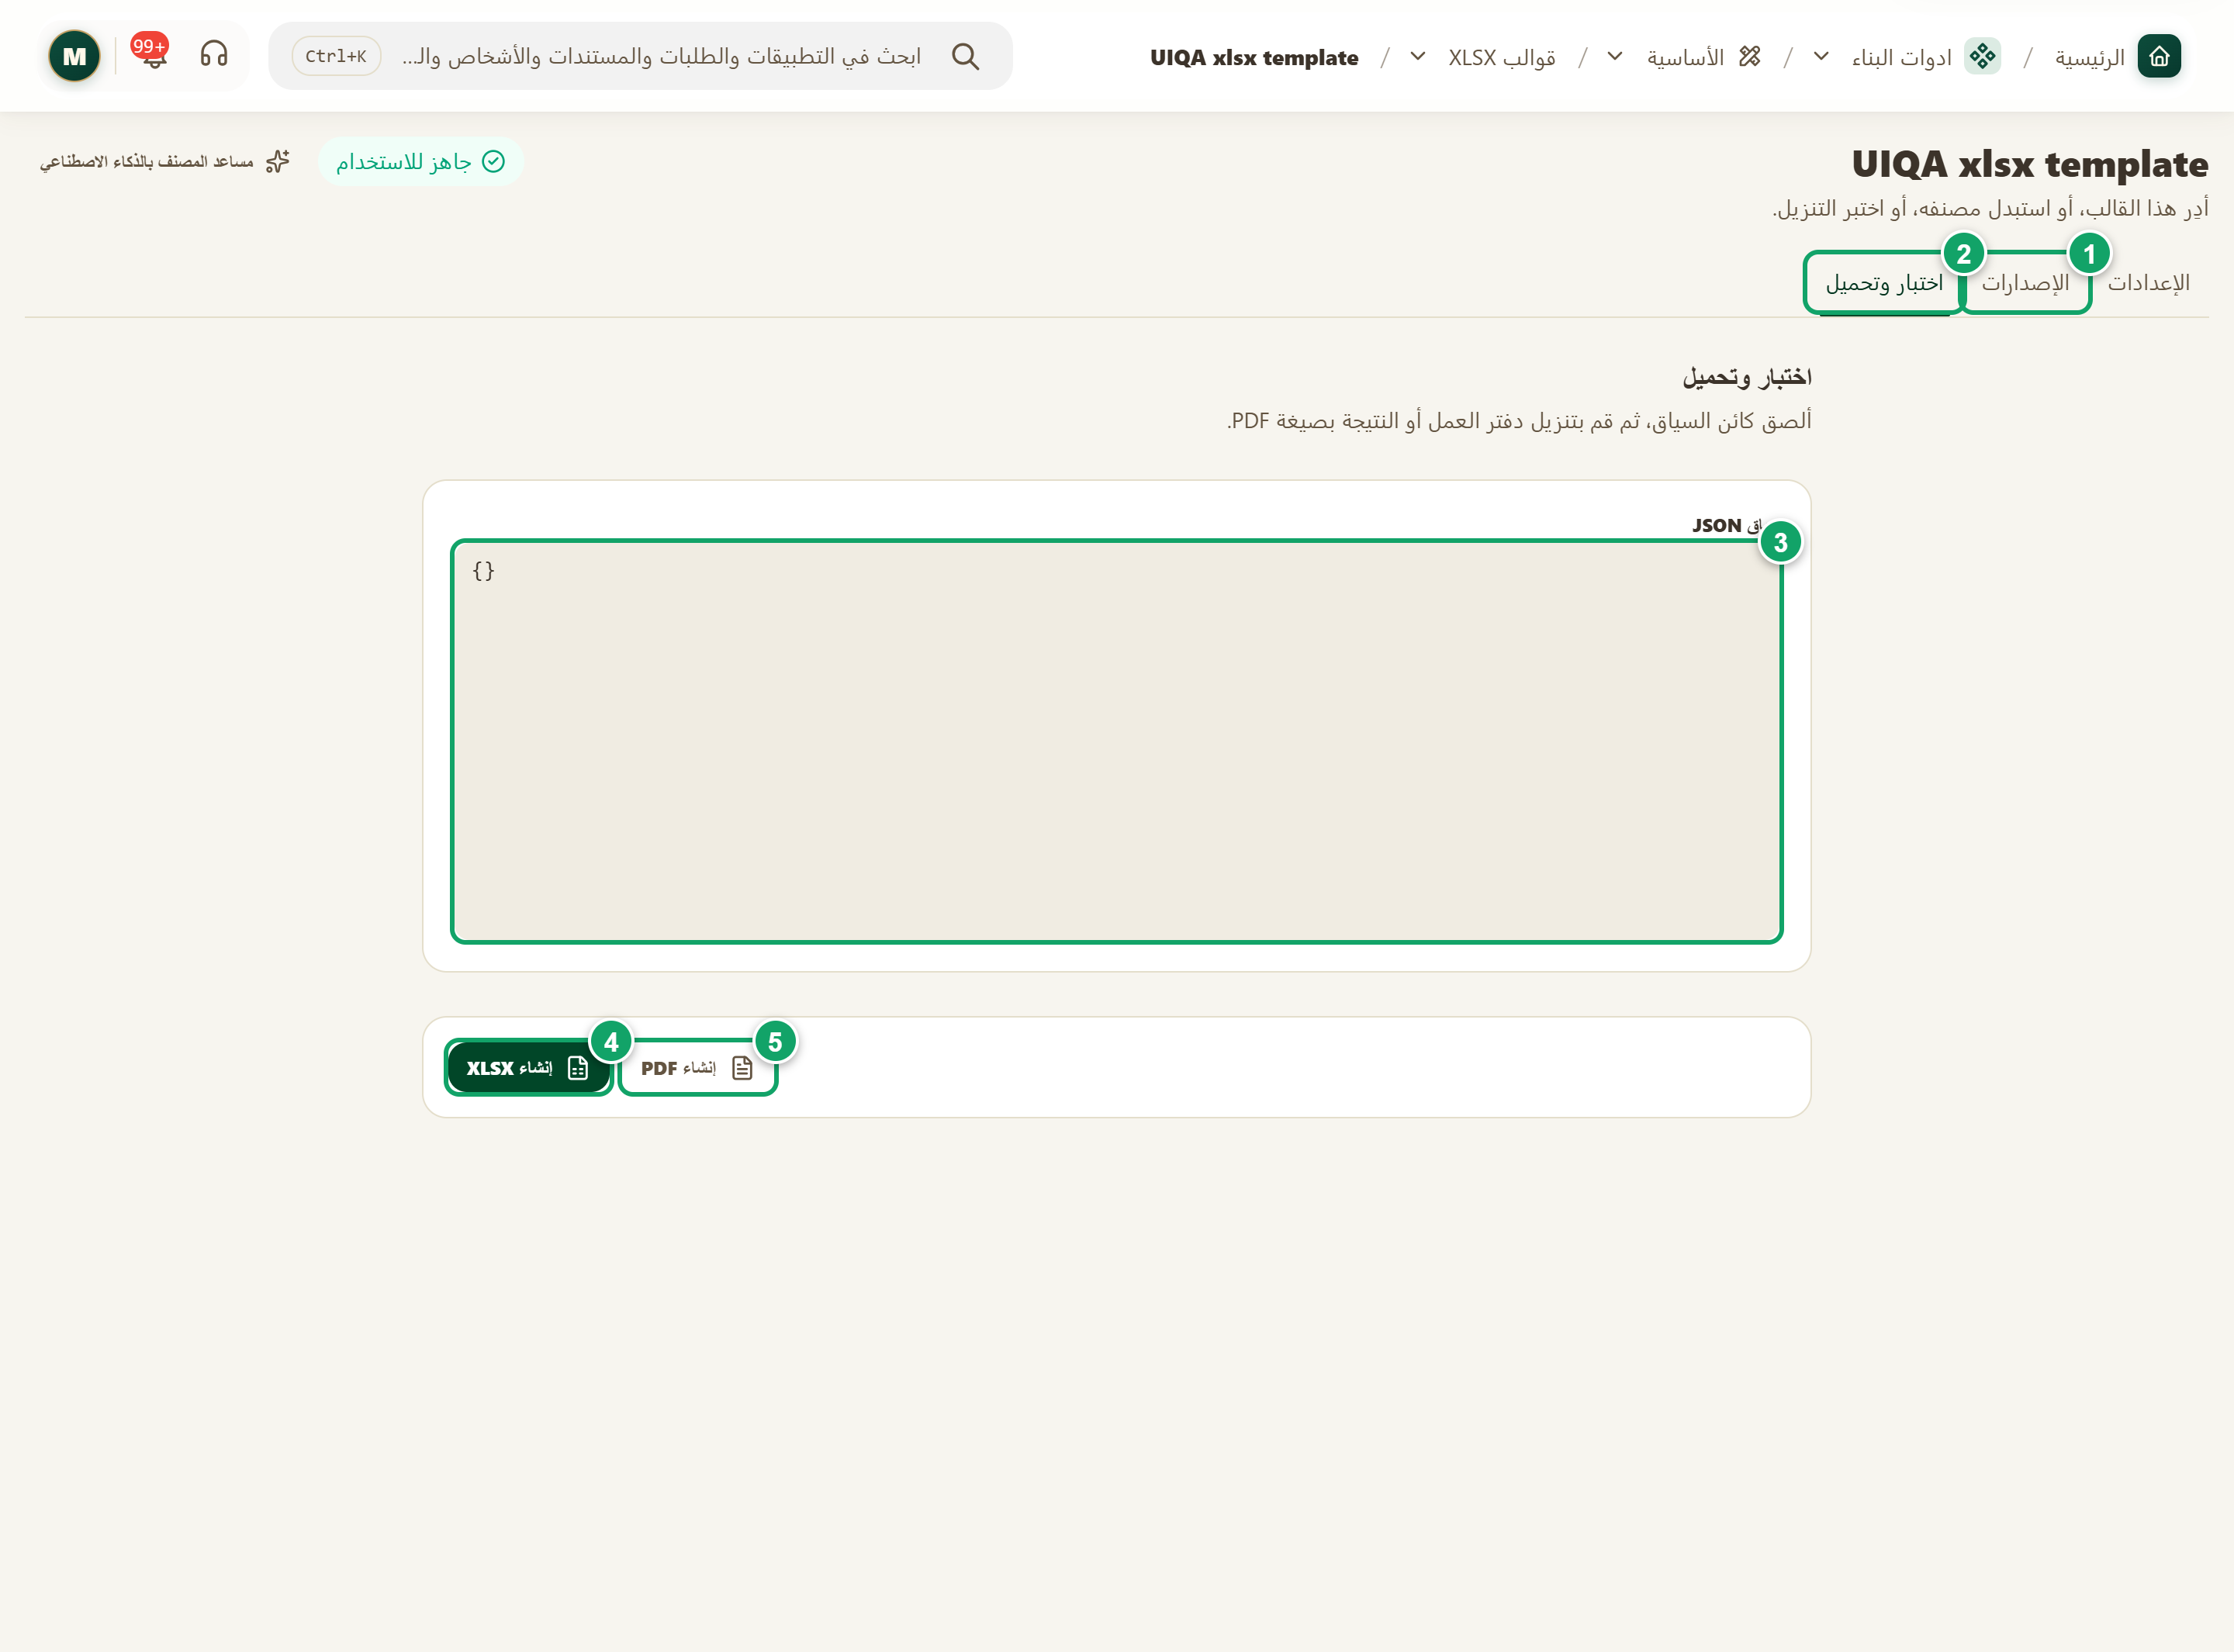
\includegraphics[width=0.95\linewidth,height=0.72\textheight,keepaspectratio]{figures/screens/ch06-xlsx-workspace-ar.png}
\caption{تبويب «اختبار وتحميل» في مساحة عمل قالب XLSX}
\label{fig:builder-xlsx-workspace-screen}
\shotnote{تعرض الصورة قالب XLSX اختبارياً في test2 مفتوحاً على «اختبار وتحميل»، ومربع السياق فيه فارغ إلا من القوسين. ويبيّن ذلك أن اختبار المصنف يعتمد على بيانات تكتبها بنفسك بصيغة JSON، لا على سجل تختاره كما في قوالب DOCX. ① «الإصدارات»: ترفع منه المصنف البديل. ② «اختبار وتحميل»: التبويب المعروض. ③ «سياق JSON»: تكتب فيه كائناً يحمل \en{\$record} وحقوله. ④ «إنشاء XLSX»: ينزّل ملف Excel لمراجعة الصفوف والصيغ. ⑤ «إنشاء PDF»: ينزّل ملف PDF لمراجعة الصفحات.}
\end{figure}

\begin{table}[H]
\centering
\caption{تبويبات مساحة العمل}
\label{tab:builder-xlsx-workspace-tabs}
\begin{tabularx}{\linewidth}{R{3.6cm} Y}
\rcHeaderRow
\thh{التبويب} & \thh{المحتوى والإجراء}\\
الإعدادات & «اسم القالب» و«الوصف» و«صيغة اسم الملف عند التنزيل» و«أذونات البيانات»، ثم «حفظ الإعدادات».\\
الإصدارات & في «استبدال المصنف» تختار ملفاً وتضغط زر التحقق والرفع، فلا يصبح حالياً إلا إذا نجح التحقق، وإلا ظهر «لم يُرفع هذا المصنف». ويعرض «سجل الإصدارات» الإصدارات من الأحدث مع علامة «الحالي».\\
اختبار وتحميل & تكتب بيانات الاختبار في «سياق JSON»، ثم تضغط «إنشاء XLSX» أو «إنشاء PDF» فيُنزَّل الملف.\\
مساعد المصنف & تكتب «تعليمات» تصف التغيير، وتؤكد إرسال سياق المصنف إلى مزود الذكاء الاصطناعي، ثم تضغط «إنشاء مسودة». وتراجعها بـ «تنزيل معاينة XLSX» و«مراجعة PDF»، ثم تضغط «اعتماد الإصدار» و«تأكيد الموافقة»، أو «حذف المسودة».\\
\end{tabularx}
\end{table}

\begin{table}[H]
\centering
\caption{ما الذي تراجعه في الملف الناتج؟}
\label{tab:builder-xlsx-workspace-checks}
\begin{tabularx}{\linewidth}{R{3.6cm} Y}
\rcHeaderRow
\thh{المراجعة} & \thh{النتيجة المتوقعة}\\
عدد الصفوف والأعمدة & يساوي عدد العناصر، مع الحفاظ على تنسيق الصف وعرض العمود.\\
الأنواع & تبقى الأرقام أرقاماً، والقيم المنطقية قيماً منطقية.\\
الصيغ والمخططات & تشير إلى النطاق الموسّع، وتظهر القيم الصحيحة بعد فتح الملف.\\
ملف PDF & منطقة الطباعة والهوامش والاتجاه وفواصل الصفحات والنص العربي سليمة.\\
\end{tabularx}
\end{table}

\begin{rcwarn}[المساعد لا يكتب فوق تعديل أحدث]
يحدد المساعد لكل تعديل الورقة والخلية ومحتواها المتوقع. فإذا تغيّر المصنف بعد الاقتراح فشل الاعتماد بدلاً من أن يكتب فوق الخلية الأحدث. ولا يعمل الاعتماد أيضاً قبل حل أسئلة ربط البيانات التي يطرحها المساعد.
\end{rcwarn}

\begin{figure}[H]
\centering
\begin{tikzpicture}[node distance=0.5cm]
\node[stepBox] (a) {\RL{فتح القالب}};
\node[stepBox,below=of a] (b) {\RL{استبدال المصنف أو}\\\RL{مسودة من المساعد}};
\node[stepBox,below=of b] (c) {\RL{التحقق من المصنف}};
\node[stepBox,below=of c] (d) {\RL{الاختبار بسياق JSON}};
\node[stepBox,below=of d] (e) {\RL{مراجعة XLSX وPDF}};
\draw[flowsTo] (a) -- (b);
\draw[flowsTo] (b) -- (c);
\draw[flowsTo] (c) -- (d);
\draw[flowsTo] (d) -- (e);
\end{tikzpicture}
\rclegend
\caption{دورة تحديث قالب XLSX}
\label{fig:builder-xlsx-workspace-flow}
\shotnote{يبيّن المخطط أن كل إصدار جديد يمر بالتحقق قبل أن يصبح حالياً، سواء رفعته بنفسك أو اعتمدته من المساعد. ثم يأتي الاختبار بالصيغتين، لأن نجاح ملف Excel لا يعني أن خدمة التحويل إلى PDF أنتجت صفحات سليمة.}
\end{figure}

\subsection{خطوات العمل والتحقق}
\begin{enumerate}
\item افتح القالب، وعدّل ما تحتاج إليه في «الإعدادات»، ثم اضغط «حفظ الإعدادات».
\item لاستبدال المصنف، افتح «الإصدارات» واختر الملف الجديد في «استبدال المصنف»، ثم اضغط زر التحقق والرفع.
\item افتح «اختبار وتحميل»، واكتب في «سياق JSON» كائناً فيه \en{\$record} وحقوله، مثل \en{\{"\$record": \{"total": 12\}\}}.
\item اضغط «إنشاء XLSX» وراجع الصفوف والصيغ، ثم اضغط «إنشاء PDF» وراجع الصفحات.
\end{enumerate}

\textbf{تحقق ومعالجة المشكلة:} يجب أن تظهر رسالة «تم تحميل نسخة XLSX.» وأن يحمل الإصدار الجديد علامة «الحالي». فإذا ظهر «أدخل كائن JSON صالح.»، فتأكد من أن النص يبدأ بقوس معقوص وينتهي به. وإذا نجح ملف Excel وفشل PDF، فالمشكلة في خدمة التحويل لا في القالب، فاطلب من مسؤول النظام التحقق منها.

\clearpage
\section{قوالب الطباعة}
\label{sec:builder-feature-print-templates}

قالب الطباعة مستند تصممه داخل كيان بالسحب والإفلات، دون أن ترفع ملف Word. ويطبع طلبات نموذج أو سجلات نوع معين بصيغة PDF أو Word، على ترويسة المؤسسة وهويتها. وتعرض صفحة «قوالب الطباعة» كل القوالب الموجودة وحالتها، أما إنشاء قالب جديد فيتم من داخل منشئ النموذج أو نوع السجلات بالضغط على «طباعة».

\textbf{المسار ومن يستخدمه:} «ادوات البناء» ← «الأساسية» ← «قوالب الطباعة». يستخدمها من يبني النماذج وأنواع السجلات.

\begin{rcnote}[مثال: شركة الأفق]
يفتح مسؤول النظام نوع «طلبات الزيارة» ويضغط «طباعة»، ثم يختار «ابدأ من نوع السجل هذا» ليصمم ورقة زيارة فيها رمز QR للتحقق، وينشرها فتظهر في زر «طباعة» داخل كل طلب. ويصل إلى القالب من ③.
\end{rcnote}

\begin{figure}[H]
\centering
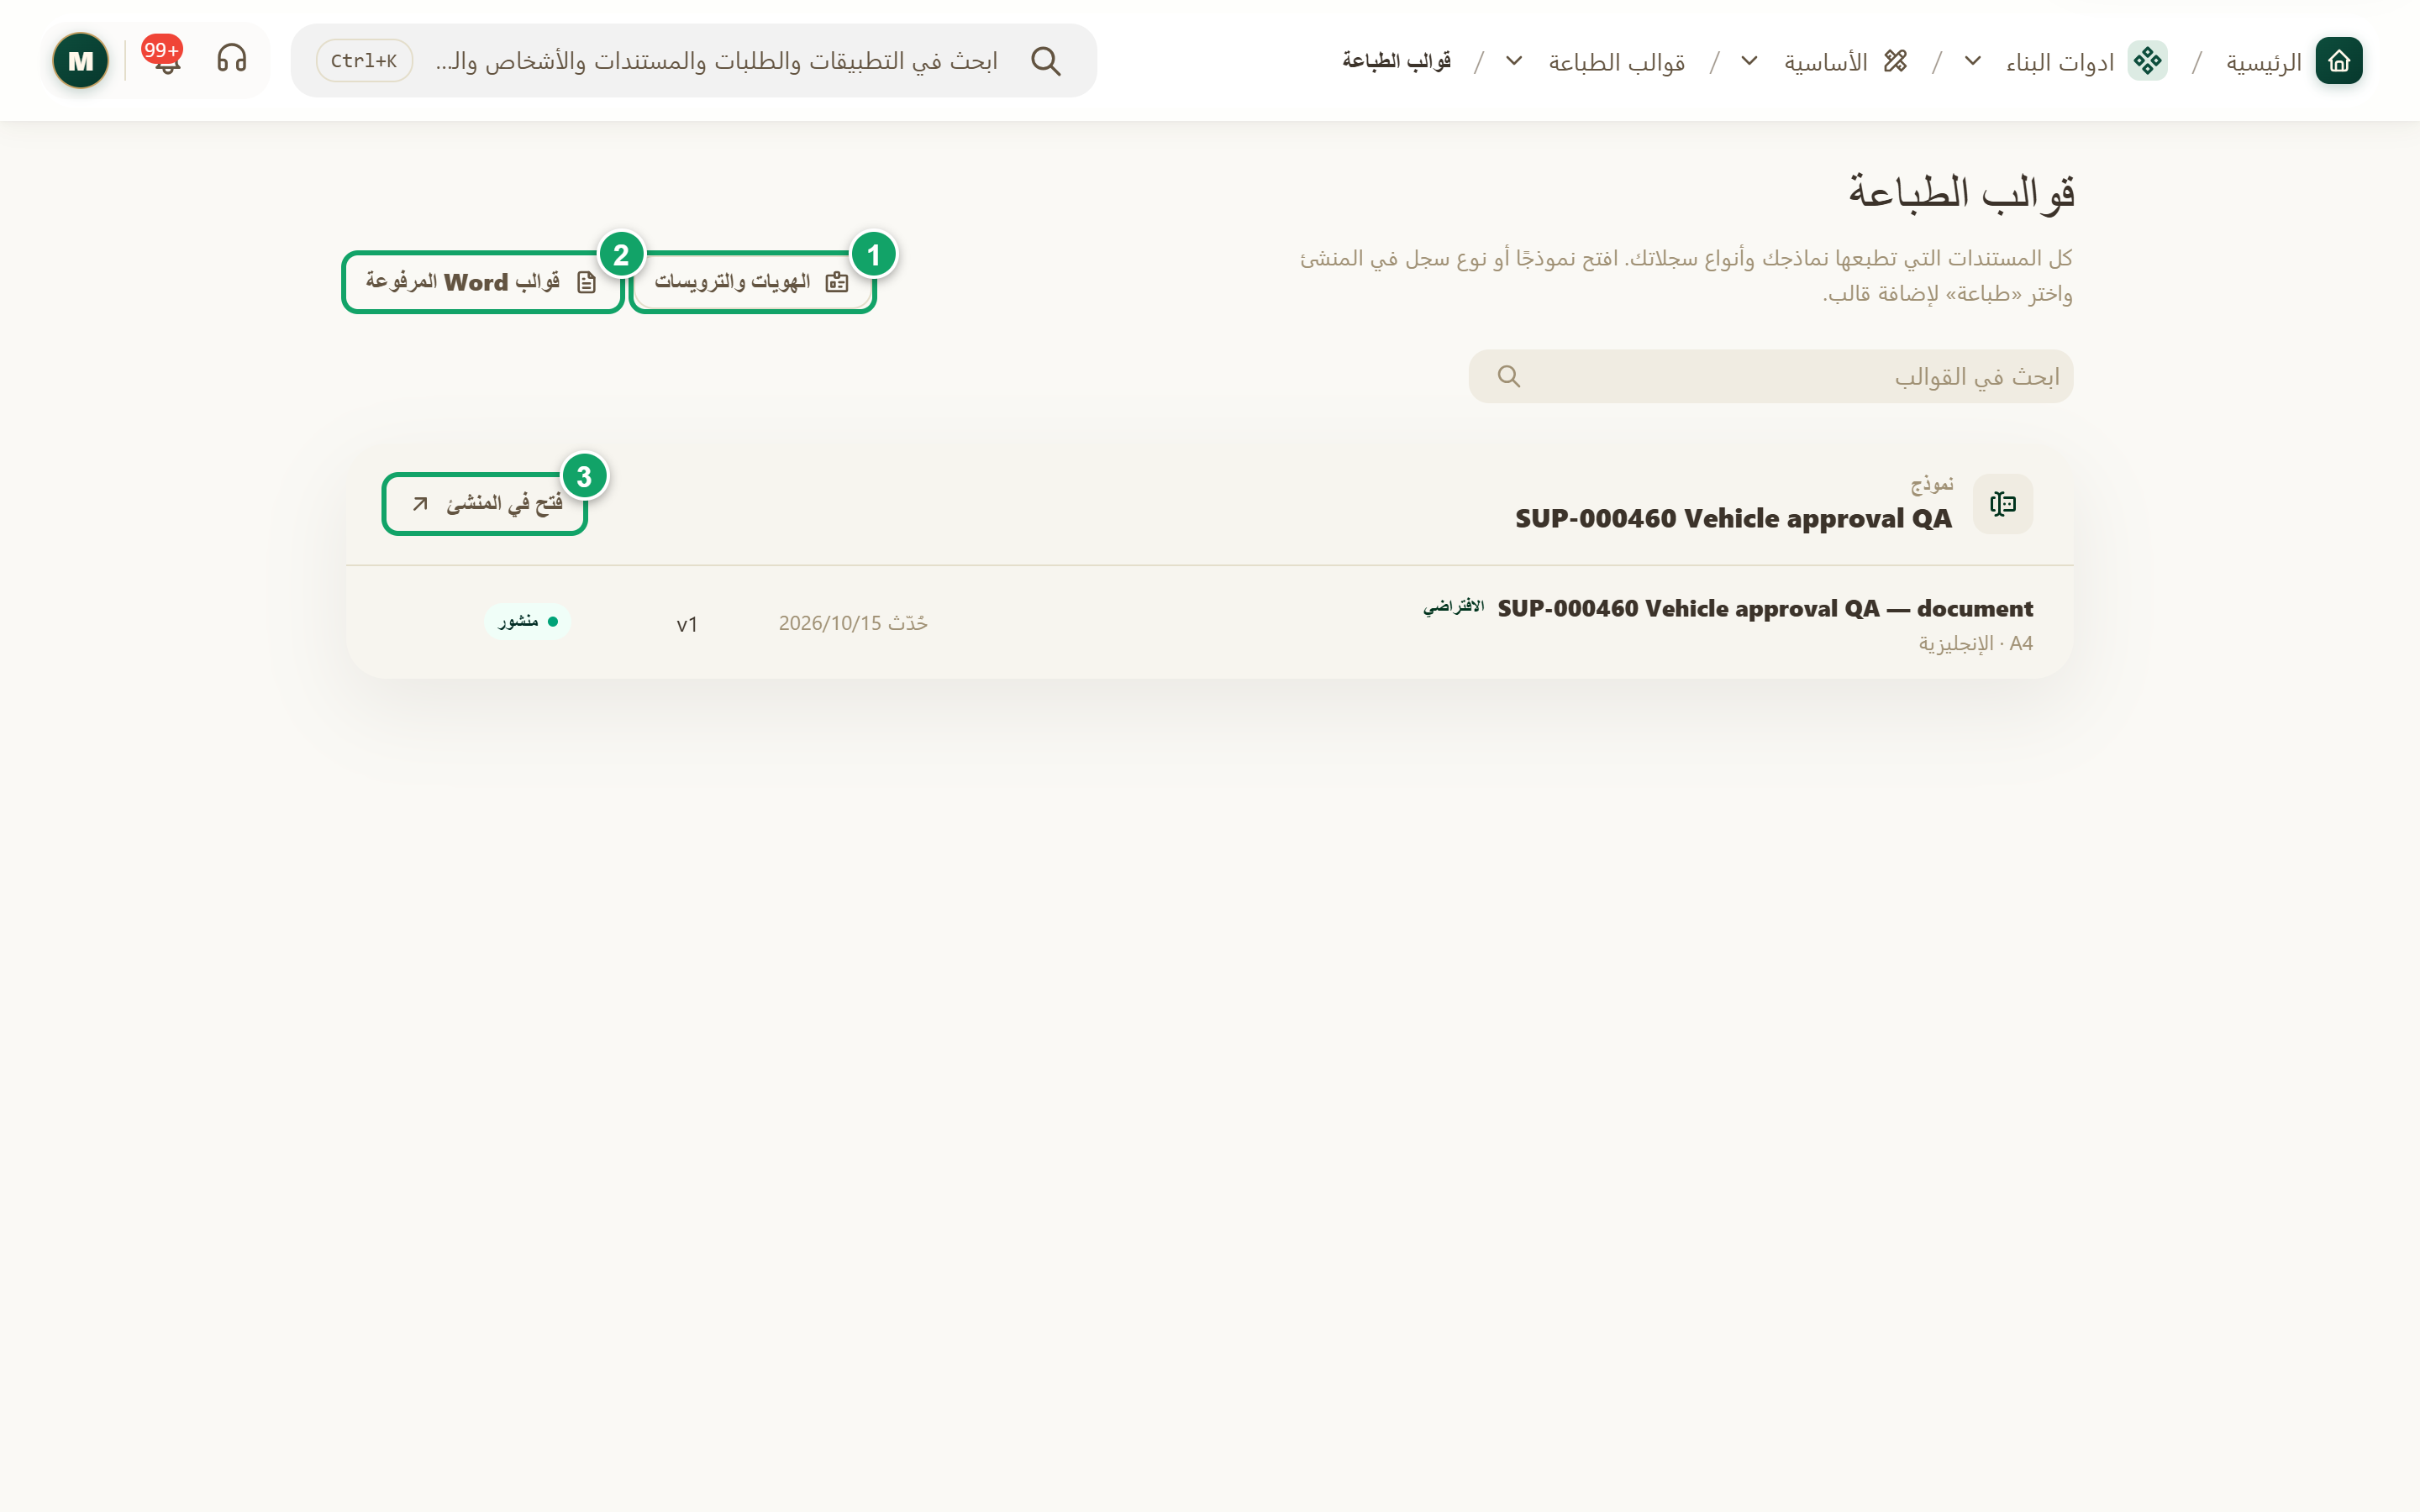
\includegraphics[width=0.95\linewidth,height=0.72\textheight,keepaspectratio]{figures/screens/ch06-print-ar.png}
\caption{مكتبة «قوالب الطباعة»}
\label{fig:builder-print-templates-screen}
\shotnote{تعرض الصفحة قوالب الطباعة مجمّعة حسب النموذج أو نوع السجلات، مع حالتها. والقالب الظاهر قالب اختبار. ① «الهويات والترويسات»: ينتقل إلى الشعارات والترويسات. ② «قوالب Word المرفوعة»: ينتقل إلى قوالب DOCX. ③ «فتح في المنشئ»: يفتح النموذج أو النوع حيث يُعدَّل القالب.}
\end{figure}


\begin{table}[H]
\centering
\caption{ما الذي تجده هنا؟}
\label{tab:builder-print-data}
\begin{tabularx}{\linewidth}{R{3.6cm} Y}
\rcHeaderRow
\thh{الجزء} & \thh{المحتوى والإجراء}\\
مكتبة القوالب & القوالب مجمّعة حسب النموذج أو نوع السجل، مع الحجم واللغة والإصدار والحالة: «منشور» أو «مسودة» أو «تغييرات غير منشورة»، وزر «فتح في المنشئ».\\
نافذة «قوالب الطباعة» & تفتح بزر «طباعة» في منشئ النموذج أو النوع، وتعرض لكل قالب «يُطبع من»: «قائمة الطباعة» أو «الطباعة الجماعية» أو «لا يظهر قبل النشر». ومنها «فتح» و«اجعله الافتراضي» و«أرشفة».\\
قالب جديد & من النافذة نفسها: «ابدأ من هذا النموذج» أو «ابدأ من نوع السجل هذا» أو «صفحة فارغة على ترويسة الجهة».\\
المخرجات & الصيغ المتاحة للتنزيل، واسم الملف، و«من يمكنه الطباعة»، والاحتفاظ بنسخة في السجل، وصفحة تحقق يفتحها رمز QR.\\
\end{tabularx}
\end{table}

\begin{figure}[H]
\centering
\begin{tikzpicture}[node distance=0.5cm]
\node[stepBox] (a) {\RL{طباعة من منشئ النموذج أو النوع}};
\node[stepBox,below=of a] (b) {\RL{تصميم البيانات والعناصر}};
\node[stepBox,below=of b] (c) {\RL{معاينة بسجل}};
\node[stepBox,below=of c] (d) {\RL{نشر}};
\node[stepBox,below=of d] (e) {\RL{زر طباعة في السجل}};
\draw[flowsTo] (a) -- (b);
\draw[flowsTo] (b) -- (c);
\draw[flowsTo] (c) -- (d);
\draw[flowsTo] (d) -- (e);
\end{tikzpicture}
\rclegend
\caption{من التصميم إلى زر الطباعة}
\label{fig:builder-print-flow}
\shotnote{يبيّن المخطط أن القالب يولد داخل منشئ النموذج أو نوع السجلات، لا في صفحة المكتبة، وأنه لا يظهر للمستخدمين قبل النشر. وتأتي المعاينة بسجل حقيقي قبل النشر لتكشف الحقول الفارغة أو الجداول الطويلة قبل أن يطبعها أحد.}
\end{figure}

\subsection{خطوات العمل والتحقق}
\begin{enumerate}
\item افتح النموذج أو نوع السجلات في المنشئ، واضغط «طباعة»، ثم اختر نقطة البداية.
\item أضف الحقول والعناصر، واضبط في «الصفحة» الورق والهوية والترويسة.
\item اضغط «معاينة بسجل» و«تنزيل ملف PDF تجريبي»، ثم حدد «من يمكنه الطباعة» واضغط «نشر».
\end{enumerate}

\textbf{تحقق ومعالجة المشكلة:} يجب أن يظهر القالب «منشور» في المكتبة، وأن يظهر في قائمة «اختر مستندًا» عند الضغط على «طباعة» في السجل. فإذا لم يظهر، فتأكد من نشره، لأن القالب «لا يظهر قبل النشر»؛ واستخدم «الفحص على جميع السجلات» لاكتشاف السجلات التي تنقصها بيانات.

\clearpage
\section{منشئ قالب الطباعة: البيانات والعناصر}
\label{sec:builder-feature-print-builder}

يفتح المنشئ عندما تختار نقطة بداية لقالب جديد أو تضغط «فتح» بجانب قالب موجود. وتظهر في وسطه الصفحة كما ستُطبع، وإلى جانبها ثلاثة تبويبات: «البيانات» و«العناصر» و«الصفحة»، وفي الجانب الآخر «الإعدادات» الخاصة بما تحدده على الصفحة. ويحفظ المنشئ عملك تلقائياً، فترى «جارٍ الحفظ…» ثم «تم الحفظ»، لكن التعديلات تبقى مسودة لا يراها أحد حتى تنشرها. وكل عنصر على الصفحة نص حقيقي في ملف PDF يمكن تحديده والبحث فيه، وليس صورة للصفحة.

\textbf{المسار ومن يستخدمه:} منشئ النموذج أو نوع السجلات ← «طباعة» ← نقطة بداية أو «فتح». يستخدمه من يبني النموذج أو نوع السجلات.

\begin{rcnote}[مثال: شركة الأفق]
يسحب مسؤول النظام حقل تاريخ الزيارة من مجموعة «هذا السجل» إلى ورقة الزيارة، ويختار له في «عندما يكون فارغًا» خيار «إيقاف الطباعة». ثم يضيف عنصر «إظهار عند» حول فقرة ملاحظات المراجعة، فلا تُطبع إلا إذا كتبت سارة الخطيب ملاحظة. ويأخذ الحقل من ①، وعنصر «إظهار عند» من ② ثم ③.
\end{rcnote}

\begin{figure}[H]
\centering
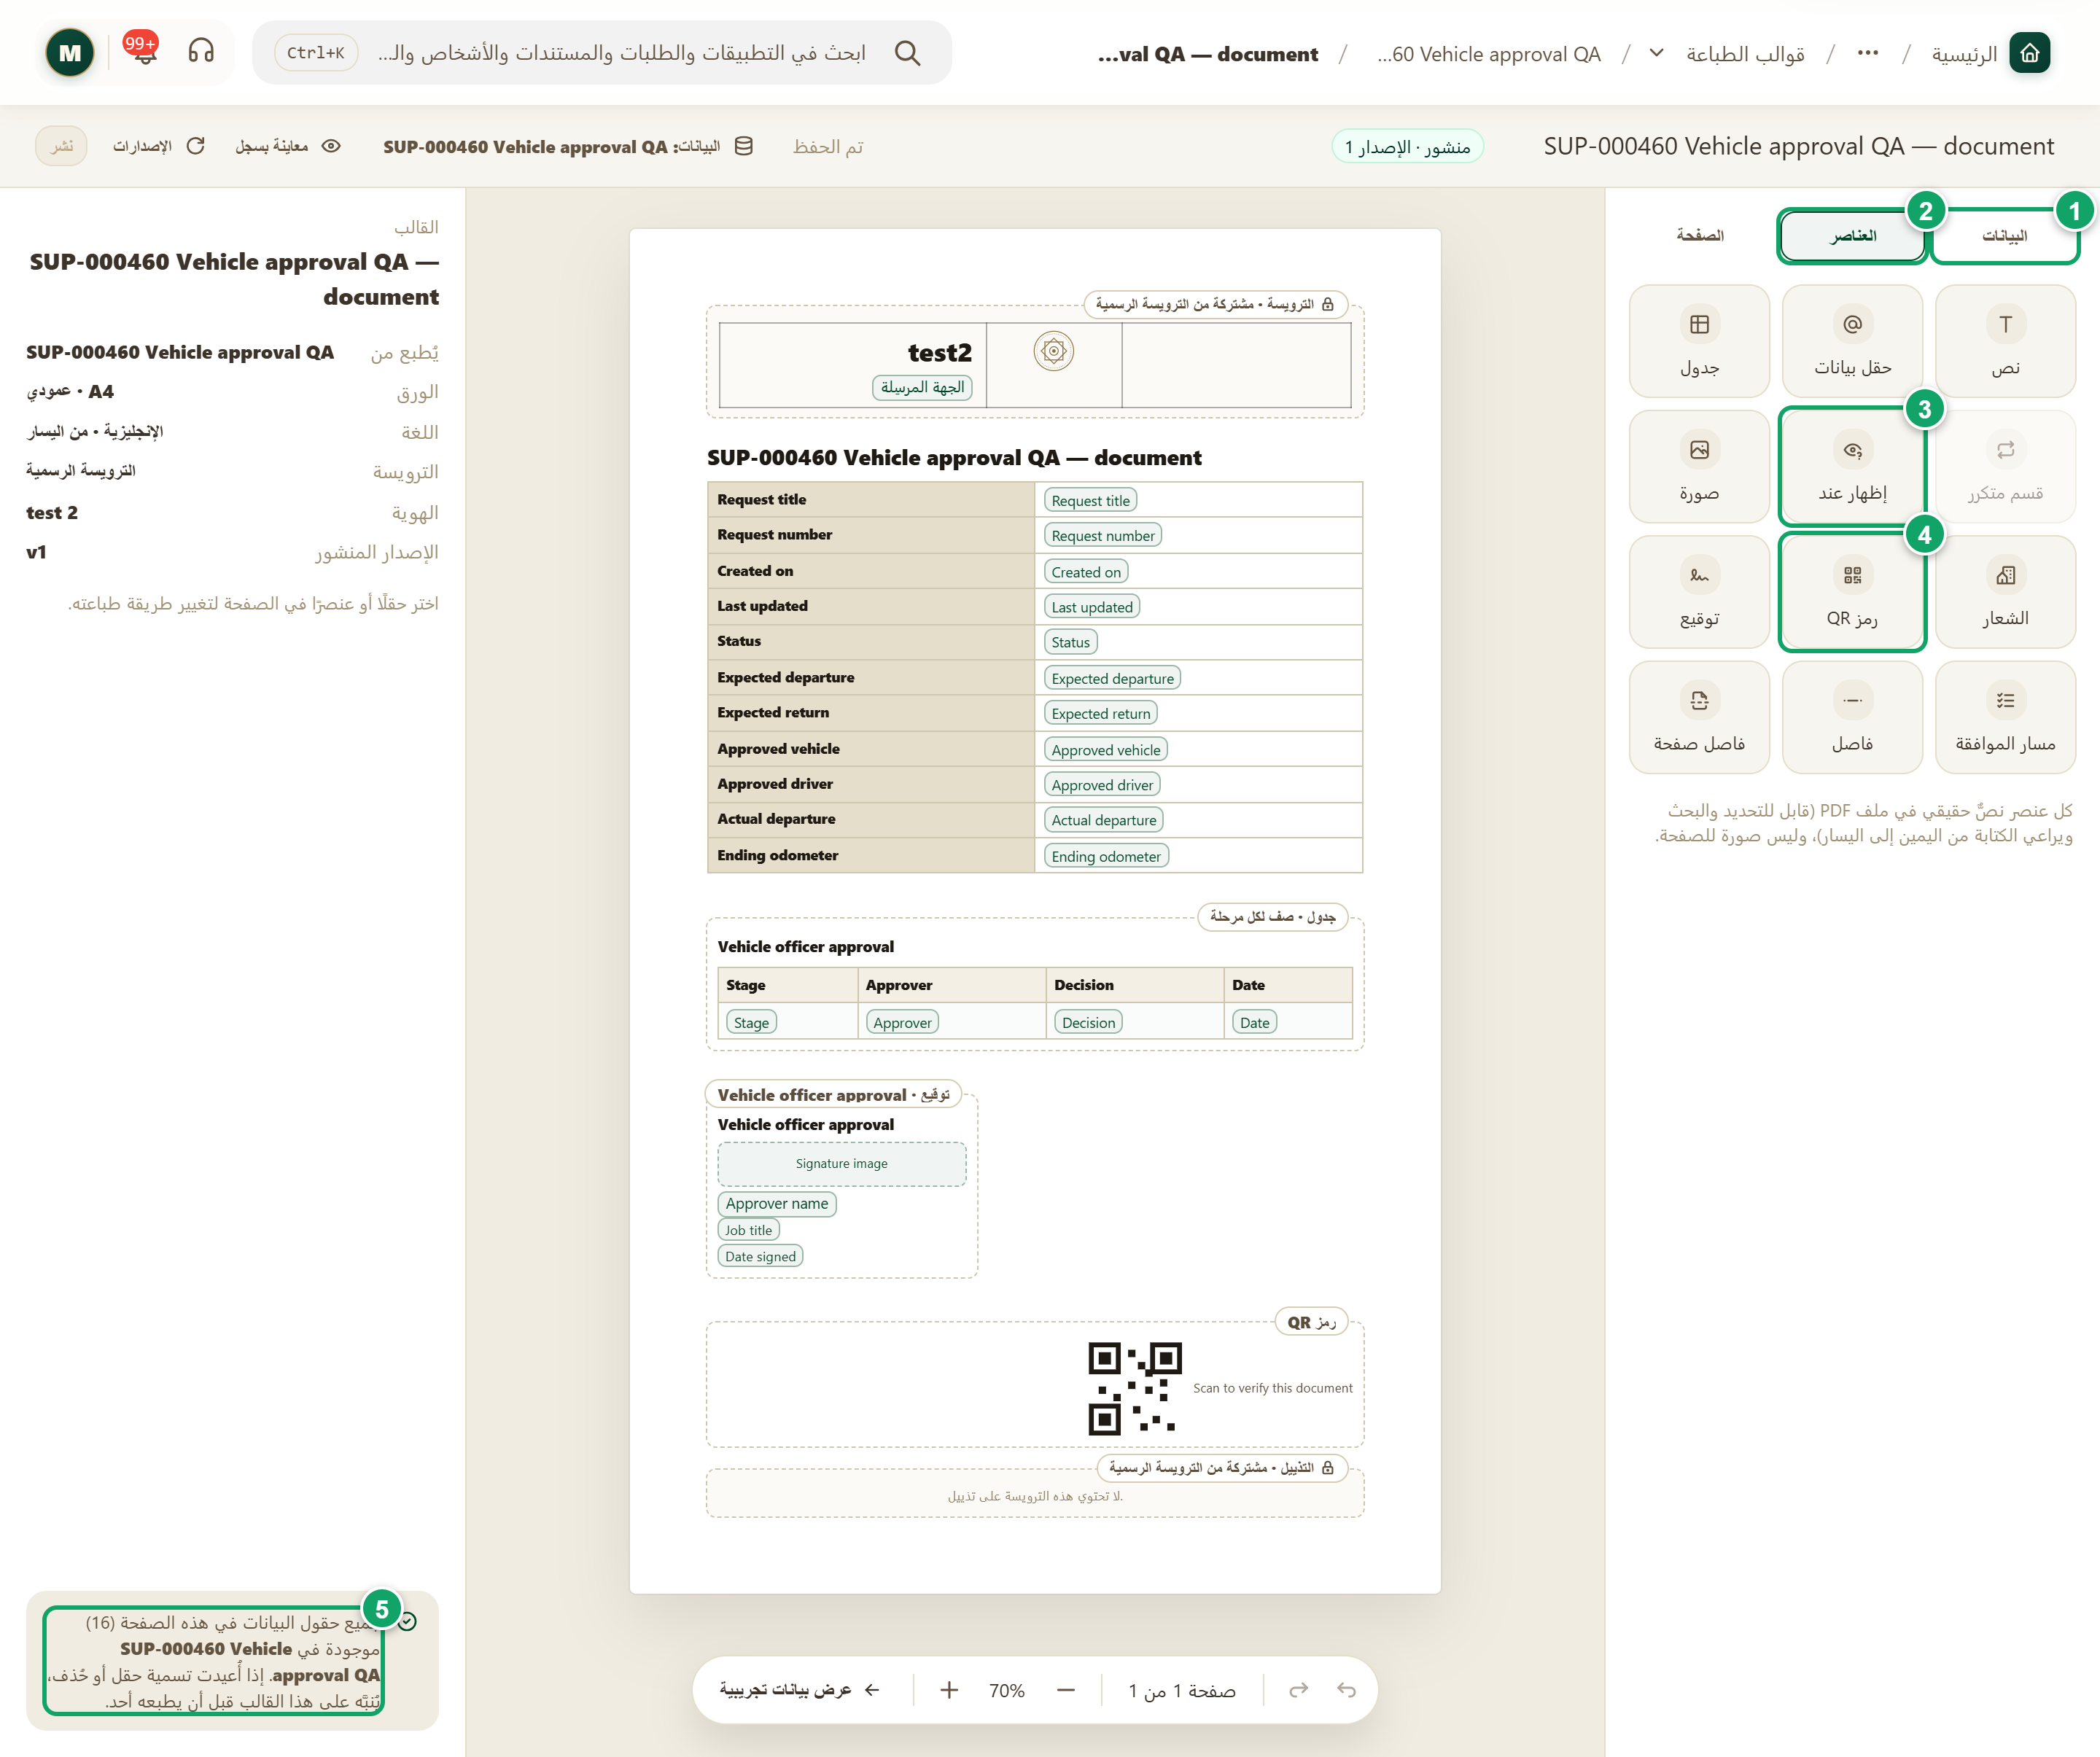
\includegraphics[width=0.95\linewidth,height=0.72\textheight,keepaspectratio]{figures/screens/ch06-print-builder-ar.png}
\caption{منشئ قالب الطباعة وتبويب «العناصر» مفتوح}
\label{fig:builder-print-builder-screen}
\shotnote{تعرض الصورة قالب طباعة اختبارياً لنموذج في test2 داخل المنشئ، والصفحة في الوسط كما ستُطبع بحقولها وجدول الموافقات والتوقيع ورمز QR. ويظهر «قسم متكرر» باهتاً لأن هذا النموذج لا يحتوي على قوائم، والعنصر لا يعمل إلا مع قائمة. ① «البيانات»: الحقول التي تسحبها إلى الصفحة. ② «العناصر»: التبويب المعروض. ③ «إظهار عند»: جزء لا يُطبع إلا إذا تحققت شروطه. ④ «رمز QR»: رمز يفتح صفحة التحقق. ⑤ شريط الحالة: يؤكد أن جميع حقول البيانات في الصفحة ما زالت موجودة.}
\end{figure}

\begin{table}[H]
\centering
\caption{تبويب «البيانات»}
\label{tab:builder-print-builder-data}
\begin{tabularx}{\linewidth}{R{3.6cm} Y}
\rcHeaderRow
\thh{المجموعة} & \thh{ما تحتويه}\\
«هذا الطلب» أو «هذا السجل» & حقول الطلب أو السجل الذي يُطبع، ولكل حقل نوعه، مثل نص أو تاريخ أو خيار.\\
«السجلات المرتبطة» & حقول السجلات التي يرتبط بها السجل، وتفتح حقولها بالضغط على اسمها.\\
«القوائم» & القوائم التي تصلح لعنصر «قسم متكرر»، مثل إجابات الجداول والسجلات المرتبطة.\\
«الموافقات والتوقيعات» & مراحل الموافقة ومن وقّع عليها، عندما يكون للنموذج أو النوع موافقات.\\
«الجهة» و«المستند» & البيانات الرسمية للهوية، وبيانات المستند مثل التاريخ ورقم الصفحة ورمز QR للتحقق.\\
\end{tabularx}
\end{table}

تضيف الحقل بسحبه إلى الصفحة، أو بكتابة \en{/} أثناء الكتابة ثم اختيار الحقل. ولا تظهر في القائمة إلا الحقول التي تستطيع قراءتها.

\begin{table}[H]
\centering
\caption{تبويب «العناصر»}
\label{tab:builder-print-builder-blocks}
\begin{tabularx}{\linewidth}{R{3.6cm} Y}
\rcHeaderRow
\thh{العنصر} & \thh{ما يضيفه}\\
«نص» و«حقل بيانات» & فقرة جديدة، أو حقل تختاره من تبويب «البيانات».\\
«جدول» & جدول ثابت لتنسيق الصفحة.\\
«قسم متكرر» & جدول فيه صف لكل عنصر من قائمة، وتحدد أعمدته وعنوانه وما يظهر عندما تكون القائمة فارغة.\\
«إظهار عند» & جزء لا يُطبع إلا عند تحقق كل شروطه، بأداة الشروط نفسها المستخدمة في قواعد النماذج.\\
«صورة» و«الشعار» & صورة من حقل صورة في الطلب، أو شعار الهوية التي يُطبع القالب باسمها.\\
«رمز QR» & رمز يفتح صفحة التحقق من المستند عند مسحه.\\
«توقيع» و«مسار الموافقة» & خانة توقيع لمرحلة موافقة تعرض الصورة والاسم والمسمى والتاريخ، أو جدولاً بمراحل الموافقة.\\
«فاصل» و«فاصل صفحة» & خط أفقي، أو بداية صفحة جديدة.\\
\end{tabularx}
\end{table}

\subsection{إعدادات حقل البيانات}

عندما تحدد حقلاً على الصفحة تظهر إعداداته. فللتاريخ تختار «التقويم»: «ميلادي» أو «هجري» أو «كلاهما»، ثم «التنسيق». وللرقم تختار مثلاً «بفواصل (1,250)» أو «مبلغ مالي». أما «عندما يكون فارغًا» فتحدد ما يحدث للحقل الفارغ: «عرض —» أو «إخفاء السطر» أو «إيقاف الطباعة»، والخيار الأخير يمنع الطباعة ويخبر الشخص بالحقل الذي يجب تعبئته.

\begin{figure}[H]
\centering
\begin{tikzpicture}[node distance=0.5cm]
\node[stepBox] (a) {\RL{اختيار نقطة البداية}};
\node[stepBox,below=of a] (b) {\RL{سحب الحقول من البيانات}};
\node[stepBox,below=of b] (c) {\RL{إضافة العناصر}};
\node[stepBox,below=of c] (d) {\RL{ضبط إعدادات كل حقل}};
\node[stepBox,below=of d] (e) {\RL{حفظ تلقائي في المسودة}};
\draw[flowsTo] (a) -- (b);
\draw[flowsTo] (b) -- (c);
\draw[flowsTo] (c) -- (d);
\draw[flowsTo] (d) -- (e);
\end{tikzpicture}
\rclegend
\caption{تصميم محتوى قالب الطباعة}
\label{fig:builder-print-builder-flow}
\shotnote{يرتب المخطط العمل من المحتوى إلى التفاصيل: الحقول أولاً، ثم العناصر التي تنظمها، ثم طريقة طباعة كل حقل. وينتهي بالمسودة لأن الحفظ التلقائي لا يعني النشر، فلا يرى المستخدمون أي تغيير حتى تنشر القالب.}
\end{figure}

\subsection{خطوات العمل والتحقق}
\begin{enumerate}
\item افتح النموذج أو نوع السجلات في المنشئ، واضغط «طباعة»، ثم اختر نقطة بداية أو اضغط «فتح» بجانب قالب.
\item افتح «البيانات»، واسحب الحقول إلى مواضعها، أو اكتب \en{/} أثناء الكتابة لإدراج حقل.
\item افتح «العناصر»، وأضف ما تحتاج إليه، مثل «قسم متكرر» لقائمة أو «رمز QR» للتحقق.
\item حدد كل حقل مهم، واضبط تنسيقه وما يحدث عندما يكون فارغاً.
\item راجع شريط الحالة أسفل الصفحة، وتأكد من أن كل حقول البيانات موجودة.
\end{enumerate}

\textbf{تحقق ومعالجة المشكلة:} يجب أن يظهر «تم الحفظ» في رأس المنشئ، وأن يذكر شريط الحالة أن جميع حقول البيانات في الصفحة موجودة. فإذا ظهر «أحد حقول البيانات لم يعد موجودًا»، فالحقل حُذف أو أُعيدت تسميته وسيُطبع بالرمز —، فاختر حقلاً آخر أو أزله. وإذا ظهر «تعذّر الحفظ»، فاضغط «إعادة المحاولة».

\clearpage
\section{إعدادات الصفحة في قالب الطباعة}
\label{sec:builder-feature-print-page}

يضبط تبويب «الصفحة» شكل الورقة التي يُطبع عليها القالب: حجمها واتجاهها ولغتها وهوامشها، والهوية التي تحمل شعارها، والترويسة التي تظهر في رأسها وتذييلها. ويمكنه أيضاً أن يطبع علامة مائية على المستند إلى أن يُعتمد الطلب. وتسري هذه الإعدادات على هذا القالب وحده، فقالب آخر قد يستخدم ورقاً أو ترويسة مختلفة.

\textbf{المسار ومن يستخدمه:} منشئ قالب الطباعة ← «الصفحة». يستخدمه من يصمم القالب.

\begin{rcnote}[مثال: شركة الأفق]
يختار مسؤول النظام لورقة الزيارة ورقاً A4 عمودياً باللغة العربية، وترويسة الأفق التي يظهر رأسها في الصفحة الأولى فقط. ويفعّل العلامة المائية «مسودة» حتى يصل الطلب إلى حالة معتمدة، فلا تخرج ورقة غير معتمدة دون هذه العلامة. ويضبط الورق في ② و③، ويختار الترويسة تحت ⑤.
\end{rcnote}

\begin{figure}[H]
\centering
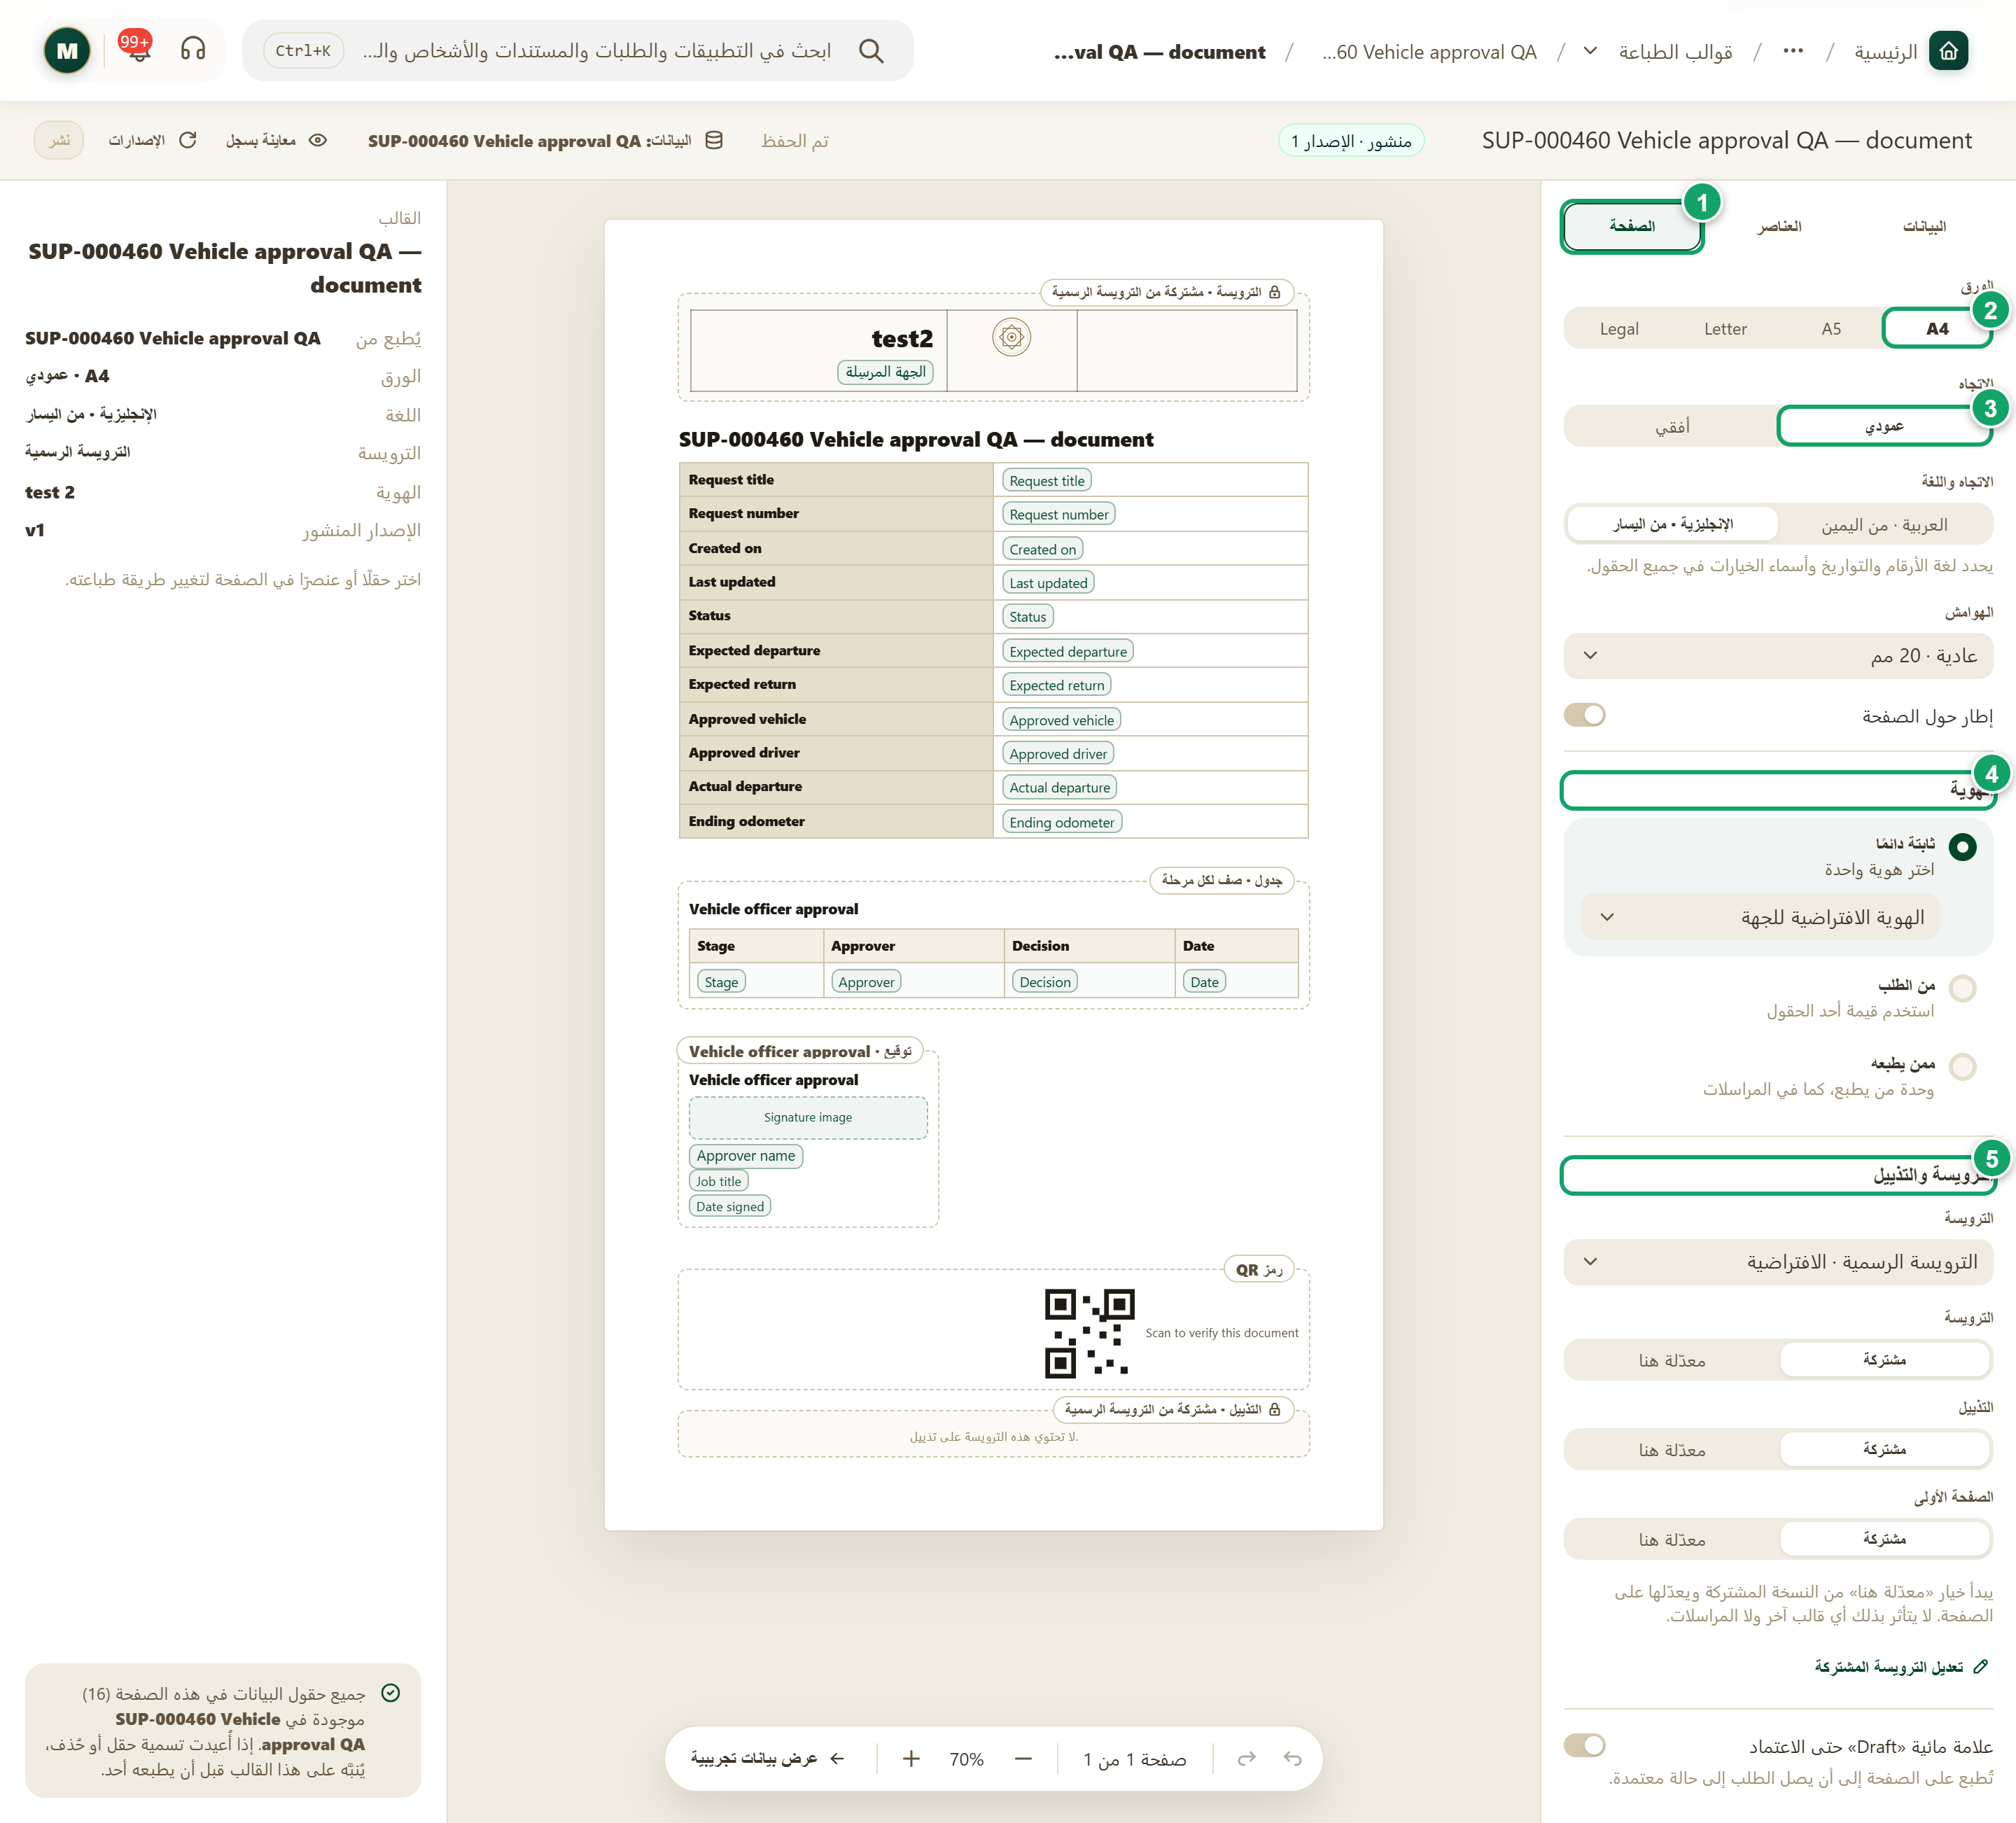
\includegraphics[width=0.95\linewidth,height=0.72\textheight,keepaspectratio]{figures/screens/ch06-print-page-ar.png}
\caption{تبويب «الصفحة» في منشئ قالب الطباعة}
\label{fig:builder-print-page-screen}
\shotnote{تعرض الصورة إعدادات الصفحة للقالب الاختباري نفسه: ورق A4 عمودي، والهوية الافتراضية للجهة، وترويسة مشتركة لم تُعدَّل في القالب. ويلخّص الجانب الآخر من المنشئ هذه الاختيارات، فتتأكد منها دون فتح كل إعداد. ① «الصفحة»: التبويب المعروض. ② «A4»: حجم الورق. ③ «عمودي»: اتجاه الورقة. ④ «الهوية»: مصدر الشعار والبيانات الرسمية. ⑤ «الترويسة والتذييل»: الترويسة المختارة، وهل تُستخدم كما هي أو تُعدَّل هنا.}
\end{figure}

\begin{table}[H]
\centering
\caption{إعدادات الورقة والهوية}
\label{tab:builder-print-page-paper}
\begin{tabularx}{\linewidth}{R{3.6cm} Y}
\rcHeaderRow
\thh{الإعداد} & \thh{الخيارات}\\
«الورق» و«الاتجاه» & A4 أو A5 أو Letter أو Legal، و«عمودي» أو «أفقي».\\
«الاتجاه واللغة» & «العربية · من اليمين» أو «الإنجليزية · من اليسار» أو «التركية · من اليسار»، وتحدد لغة الأرقام والتواريخ وأسماء الخيارات في كل الحقول.\\
«الهوامش» & «بلا هوامش» أو «ضيقة» أو «عادية» أو «عريضة» أو «مخصصة» بالمليمتر، مع خيار «إطار حول الصفحة».\\
«الهوية» & «ثابتة دائمًا» لهوية واحدة تختارها، أو «من الطلب» أو «من السجل» حسب قيمة أحد الحقول مع هوية بديلة للقيم الأخرى، أو «ممن يطبعه» حسب وحدة من يطبع.\\
العلامة المائية & «علامة مائية «مسودة» حتى الاعتماد»، وتختار في «لا علامة مائية عندما تكون الحالة» الحالات التي تختفي عندها. وإذا لم يكن للسجل حقل حالة، فتُطبع العلامة دائماً.\\
\end{tabularx}
\end{table}

\begin{table}[H]
\centering
\caption{«الترويسة والتذييل»}
\label{tab:builder-print-page-letterhead}
\begin{tabularx}{\linewidth}{R{3.6cm} Y}
\rcHeaderRow
\thh{الإعداد} & \thh{ما يفعله}\\
الترويسة & تختار ترويسة من الترويسات المشتركة، أو «بلا ترويسة».\\
«مشتركة» أو «معدّلة هنا» & تأخذ رأس الصفحة أو تذييلها من الترويسة المشتركة كما هي، أو تبدأ منها وتعدّلها على هذه الصفحة دون أن يتأثر أي قالب آخر أو المراسلات. ويعيدك «العودة إلى المشتركة» إلى الأصل.\\
الصفحات & في «تُطبع الترويسة في» و«يُطبع التذييل في» تختار «كل الصفحات» أو «الصفحة الأولى فقط».\\
تعديل الترويسة المشتركة & ينقلك إلى محرر الترويسة، وأي تعديل فيه يظهر في كل قالب يستخدمها.\\
«تغيّرت الترويسة المشتركة» & تنبيه يظهر بعد تعديل الترويسة المشتركة، ومنه «مقارنة» أو «اعتماد الجديدة» أو «الإبقاء على نسختي» للأجزاء التي عدّلتها هنا.\\
\end{tabularx}
\end{table}

\begin{figure}[H]
\centering
\begin{tikzpicture}[node distance=0.5cm]
\node[stepBox] (a) {\RL{الورق والاتجاه}};
\node[stepBox,below=of a] (b) {\RL{اللغة والهوامش}};
\node[stepBox,below=of b] (c) {\RL{الهوية}};
\node[stepBox,below=of c] (d) {\RL{الترويسة والتذييل}};
\node[stepBox,below=of d] (e) {\RL{العلامة المائية}};
\draw[flowsTo] (a) -- (b);
\draw[flowsTo] (b) -- (c);
\draw[flowsTo] (c) -- (d);
\draw[flowsTo] (d) -- (e);
\end{tikzpicture}
\rclegend
\caption{ضبط الصفحة من الورق إلى العلامة المائية}
\label{fig:builder-print-page-flow}
\shotnote{يتبع المخطط ترتيب الإعدادات في تبويب «الصفحة». وتسبق الهوية الترويسة لأن الترويسة تعرض شعار الهوية واسمها، فإذا تغيّرت الهوية تغيّر ما يظهر في رأس الصفحة.}
\end{figure}

\subsection{خطوات العمل والتحقق}
\begin{enumerate}
\item افتح تبويب «الصفحة»، واختر «الورق» و«الاتجاه»، ثم اللغة في «الاتجاه واللغة».
\item اختر الهامش المناسب، وفعّل «إطار حول الصفحة» إن احتجت إليه.
\item اختر في «الهوية» هوية ثابتة، أو اربطها بحقل في السجل إذا كان لكل فرع هوية.
\item اختر الترويسة، وحدد الصفحات التي يظهر فيها رأسها وتذييلها.
\item فعّل العلامة المائية إن أردت، واختر الحالات المعتمدة التي تختفي عندها.
\end{enumerate}

\textbf{تحقق ومعالجة المشكلة:} يجب أن تظهر الصفحة في المنشئ بالحجم والاتجاه والترويسة التي اخترتها، وأن يلخّص المنشئ الورق واللغة والترويسة والهوية. فإذا ظهر «تعذّر تحميل الترويسات وهويات الجهة»، فلا يمكن عرض القالب كما سيُطبع، فأعد المحاولة. وإذا أُرشفت الترويسة أو الهوية التي يستخدمها القالب، فاختر غيرها قبل الطباعة.

\clearpage
\section{المعاينة والنشر والطباعة من السجل}
\label{sec:builder-feature-print-publish}

قبل أن يصل القالب إلى المستخدمين تعاينه على سجل حقيقي، وتضبط مخرجاته، ثم تنشره. فزر «معاينة بسجل» في رأس المنشئ يفتح صفحة المعاينة، وفيها المستند كما سيُطبع وإعدادات «المخرجات» وزر النشر. وكل نشر ينشئ إصداراً جديداً، ويُسجَّل في كل ملف PDF الإصدار الذي أُنشئ به، فيمكن دائماً إعادة إنتاج أي نسخة مطبوعة قديمة. وبعد النشر يطبع المستخدمون المستند من زر «طباعة» في السجل.

\textbf{المسار ومن يستخدمه:} منشئ قالب الطباعة ← «معاينة بسجل». يستخدمه من يصمم القالب، أما زر «طباعة» فيستخدمه كل من يملك صلاحية الطباعة في السجل.

\begin{rcnote}[مثال: شركة الأفق]
يعاين مسؤول النظام ورقة الزيارة على الطلب HZN-VR-0001، ثم يقرأ نتيجة «الفحص على جميع السجلات» فيجد طلبين بلا تاريخ زيارة. ويختار «كل من يمكنه فتح السجل» وينشر الإصدار 1، فيطبع عمر حداد الورقة من زر «طباعة» في طلبه. فيختار الطلب من القائمة التي يبدأ بها ①، ويقرأ نتيجة الفحص فوق ②، ثم ينشر من ⑤.
\end{rcnote}

\begin{figure}[H]
\centering
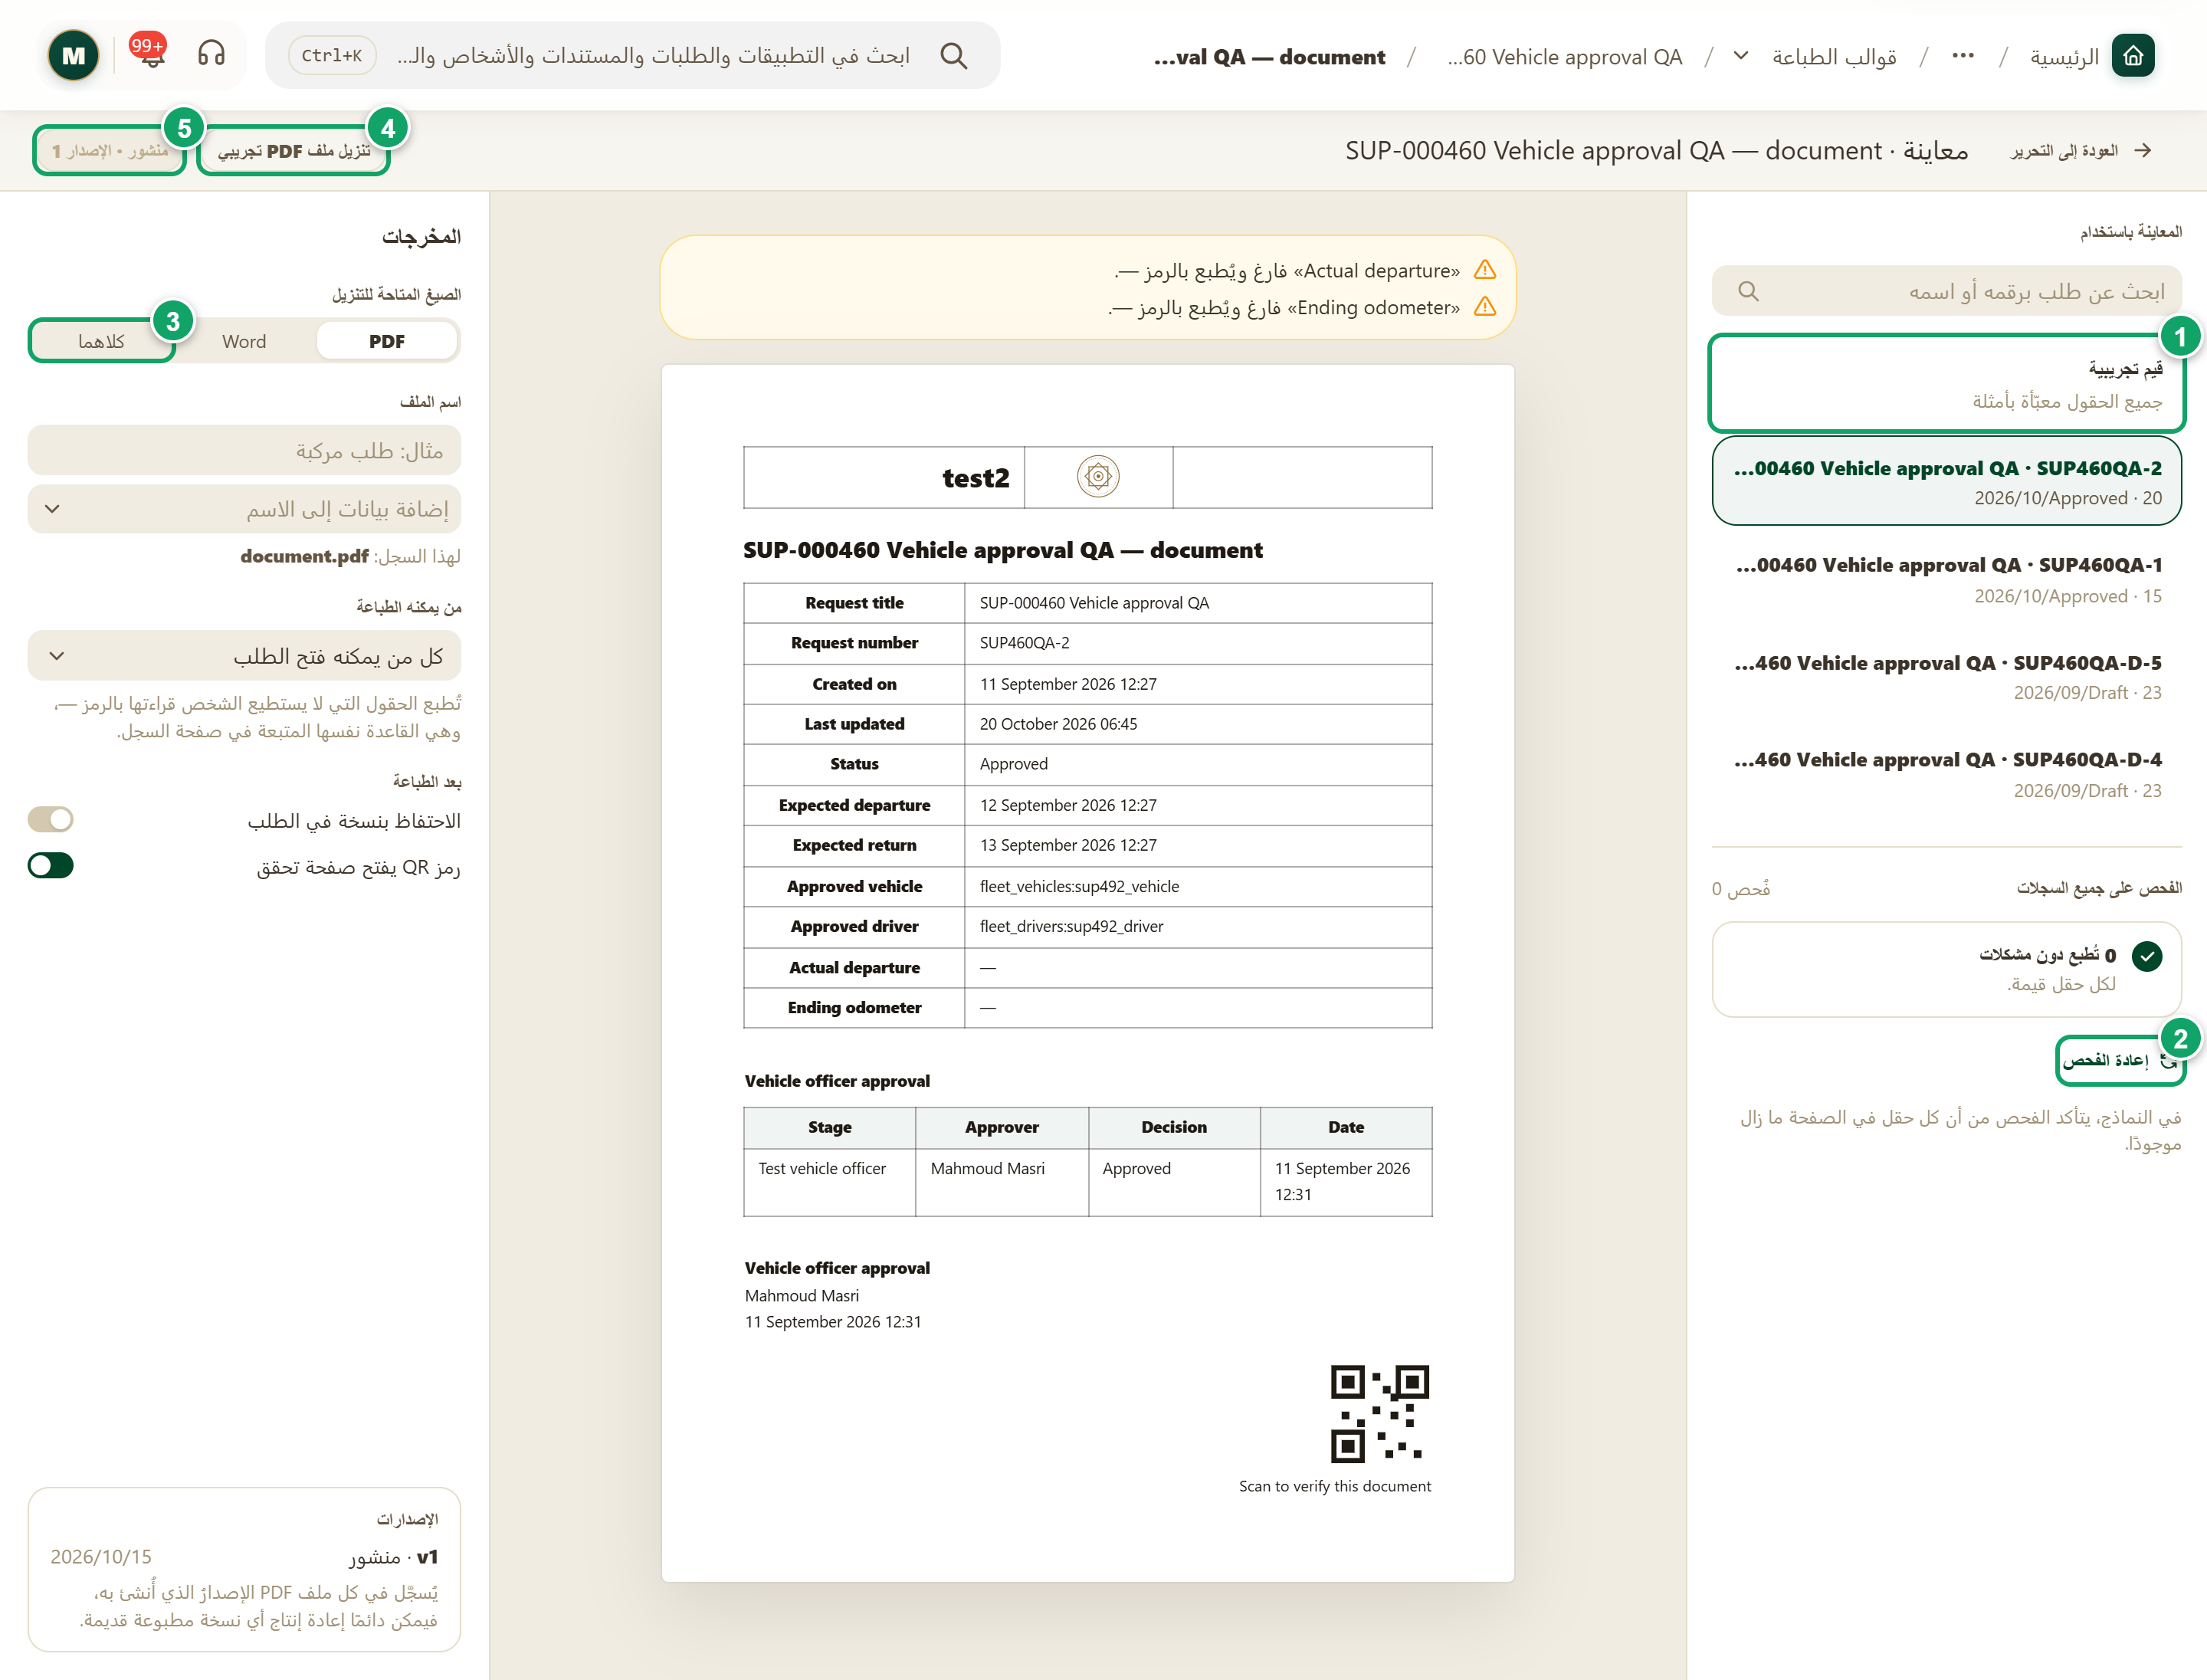
\includegraphics[width=0.95\linewidth,height=0.72\textheight,keepaspectratio]{figures/screens/ch06-print-publish-ar.png}
\caption{صفحة معاينة قالب الطباعة}
\label{fig:builder-print-publish-screen}
\shotnote{تعرض الصورة معاينة القالب الاختباري على طلب حقيقي في test2، ويظهر فوق المستند تنبيه بحقلين فارغين سيُطبعان بالرمز —. وتجمع الصفحة المعاينة والفحص والمخرجات، فتقرر النشر وأنت ترى النتيجة. ① «قيم تجريبية»: أول القائمة التي تختار منها أمثلة أو سجلاً حقيقياً. ② «إعادة الفحص»: يعيد «الفحص على جميع السجلات» بعد أي تعديل. ③ «كلاهما»: يسمح بتنزيل PDF وWord معاً. ④ «تنزيل ملف PDF تجريبي»: ينزّل المستند للسجل المختار. ⑤ زر النشر: يعرض «منشور · الإصدار 1» لأنه لا توجد تغييرات غير منشورة.}
\end{figure}

\begin{table}[H]
\centering
\caption{صفحة المعاينة}
\label{tab:builder-print-publish-preview}
\begin{tabularx}{\linewidth}{R{3.6cm} Y}
\rcHeaderRow
\thh{الجزء} & \thh{المحتوى والإجراء}\\
«المعاينة باستخدام» & تبحث عن سجل برقمه أو اسمه، أو تختار «قيم تجريبية» تملأ كل الحقول بأمثلة.\\
«الفحص على جميع السجلات» & يعمل تلقائياً عند فتح الصفحة، ويعيد زر «إعادة الفحص» تشغيله بعد أي تعديل. يفحص أحدث السجلات التي يمكنك فتحها، ويخبرك بعدد ما يُطبع دون مشكلات وبما ينقصه حقل أو يخفيه عن بعض الأشخاص. وفي النماذج يتأكد فقط من أن كل حقل ما زال موجوداً.\\
«تنزيل ملف PDF تجريبي» & ينزّل المستند للسجل المختار، ولا يعمل قبل اختيار سجل.\\
«المخرجات» & «الصيغ المتاحة للتنزيل»: PDF أو Word أو «كلاهما»؛ و«اسم الملف» مع «إضافة بيانات إلى الاسم»؛ و«من يمكنه الطباعة»: كل من يفتح السجل أو من يعدّله فقط؛ و«الاحتفاظ بنسخة في السجل»؛ و«رمز QR يفتح صفحة تحقق».\\
«نشر الإصدار N» & ينشر القالب، فتستخدم الطباعات الجديدة هذا الإصدار. ويعرض زر «الإصدارات» في رأس المنشئ الإصدارات المنشورة وتواريخها.\\
\end{tabularx}
\end{table}

\begin{table}[H]
\centering
\caption{الطباعة من السجل}
\label{tab:builder-print-publish-record}
\begin{tabularx}{\linewidth}{R{3.6cm} Y}
\rcHeaderRow
\thh{الإجراء} & \thh{ما يحدث}\\
«طباعة» ← «اختر مستندًا» & يعرض القوالب المنشورة، والقالب الافتراضي أولاً.\\
«تنزيل PDF» أو «اطبع الآن» أو «تنزيل ملف Word» & ينشئ المستند بالصيغ التي سمحت بها في «المخرجات».\\
«النسخ المطبوعة» & يعرض النسخ المحفوظة إذا فعّلت الاحتفاظ بنسخة في السجل.\\
«املأ هذه الحقول قبل الطباعة» & يظهر عندما يكون حقل مضبوط على «إيقاف الطباعة» فارغاً.\\
الطباعة الجماعية & تحدد عدة سجلات في جدول نوع السجلات وتضغط «طباعة»، ثم تختار ملف PDF واحداً أو ملف Word واحداً أو ملفاً مضغوطاً. وتُتخطّى السجلات التي لا يمكنك فتحها وتُذكر لك.\\
\end{tabularx}
\end{table}

\begin{figure}[H]
\centering
\begin{tikzpicture}[node distance=0.5cm]
\node[stepBox] (a) {\RL{معاينة بسجل}};
\node[stepBox,below=of a] (b) {\RL{الفحص على جميع السجلات}};
\node[stepBox,below=of b] (c) {\RL{ضبط المخرجات}};
\node[stepBox,below=of c] (d) {\RL{نشر الإصدار}};
\node[stepBox,below=of d] (e) {\RL{طباعة من السجل}};
\draw[flowsTo] (a) -- (b);
\draw[flowsTo] (b) -- (c);
\draw[flowsTo] (c) -- (d);
\draw[flowsTo] (d) -- (e);
\end{tikzpicture}
\rclegend
\caption{من المعاينة إلى أول نسخة مطبوعة}
\label{fig:builder-print-publish-flow}
\shotnote{يضع المخطط الفحص الشامل بعد معاينة سجل واحد، لأن سجلاً سليماً لا يضمن أن بقية السجلات تملك الحقول نفسها. ويأتي ضبط المخرجات قبل النشر، فهو الذي يحدد الصيغ ومن يطبع وما إذا كان المستند يحمل رمز تحقق.}
\end{figure}

\subsection{خطوات العمل والتحقق}
\begin{enumerate}
\item اضغط «معاينة بسجل»، وابحث عن سجل حقيقي في «المعاينة باستخدام».
\item راجع نتيجة «الفحص على جميع السجلات»، واضغط «إعادة الفحص» بعد أي تعديل، وعالج ما يظهر من حقول ناقصة أو محذوفة.
\item اضبط «المخرجات»: الصيغ، واسم الملف، و«من يمكنه الطباعة»، والاحتفاظ بنسخة، ورمز التحقق.
\item اضغط «تنزيل ملف PDF تجريبي» وراجع الملف، ثم اضغط «نشر الإصدار N».
\item افتح سجلاً، واضغط «طباعة»، واختر القالب ونزّل المستند.
\end{enumerate}

\textbf{تحقق ومعالجة المشكلة:} يجب أن تظهر رسالة «نُشر الإصدار N. ستستخدم الطباعات الجديدة هذا الإصدار.» وأن يظهر القالب في «اختر مستندًا». فإذا ظهر «تعذّر حفظ آخر تعديلاتك، لذلك لم يُنشر شيء»، فعالج مشكلة الحفظ ثم انشر مرة أخرى. وإذا طُبع حقل بالرمز —، فقد يكون فارغاً أو لا يملك الشخص صلاحية قراءته.

\clearpage
\section{صفحة التحقق من المستند}
\label{sec:builder-feature-print-verify}

عندما تفعّل «رمز QR يفتح صفحة تحقق» في مخرجات القالب، يحمل كل مستند مطبوع رمز تحقق خاصاً به. ويفتح مسح الرمز صفحة عامة لا تحتاج إلى تسجيل الدخول، تعرض المستند كما صدر وبياناته الأساسية. وبذلك يستطيع من يستلم الورقة، داخل المؤسسة أو خارجها، أن يتأكد من أنها صادرة فعلاً وأن محتواها لم يتغير. لكن الرمز يوثّق المستند الذي صدر، لا الورقة التي يظهر عليها، لذلك يقارن القارئ بين الاثنين.

\textbf{المسار ومن يستخدمه:} مسح رمز QR المطبوع على المستند، أو فتح رابطه. يستخدمها مستلم المستند، أما من يصمم القالب فيفعّلها من «المخرجات».

\begin{rcnote}[مثال: شركة الأفق]
يستلم فرع حلب ورقة الزيارة المطبوعة للطلب HZN-VR-0001، فيمسح موظف الاستقبال رمزها. فتظهر صفحة «الرمز موثّق» ومعها المستند كما صدر، فيقارن التاريخ والأسماء بالورقة التي بين يديه.
\end{rcnote}

\begin{figure}[H]
\centering
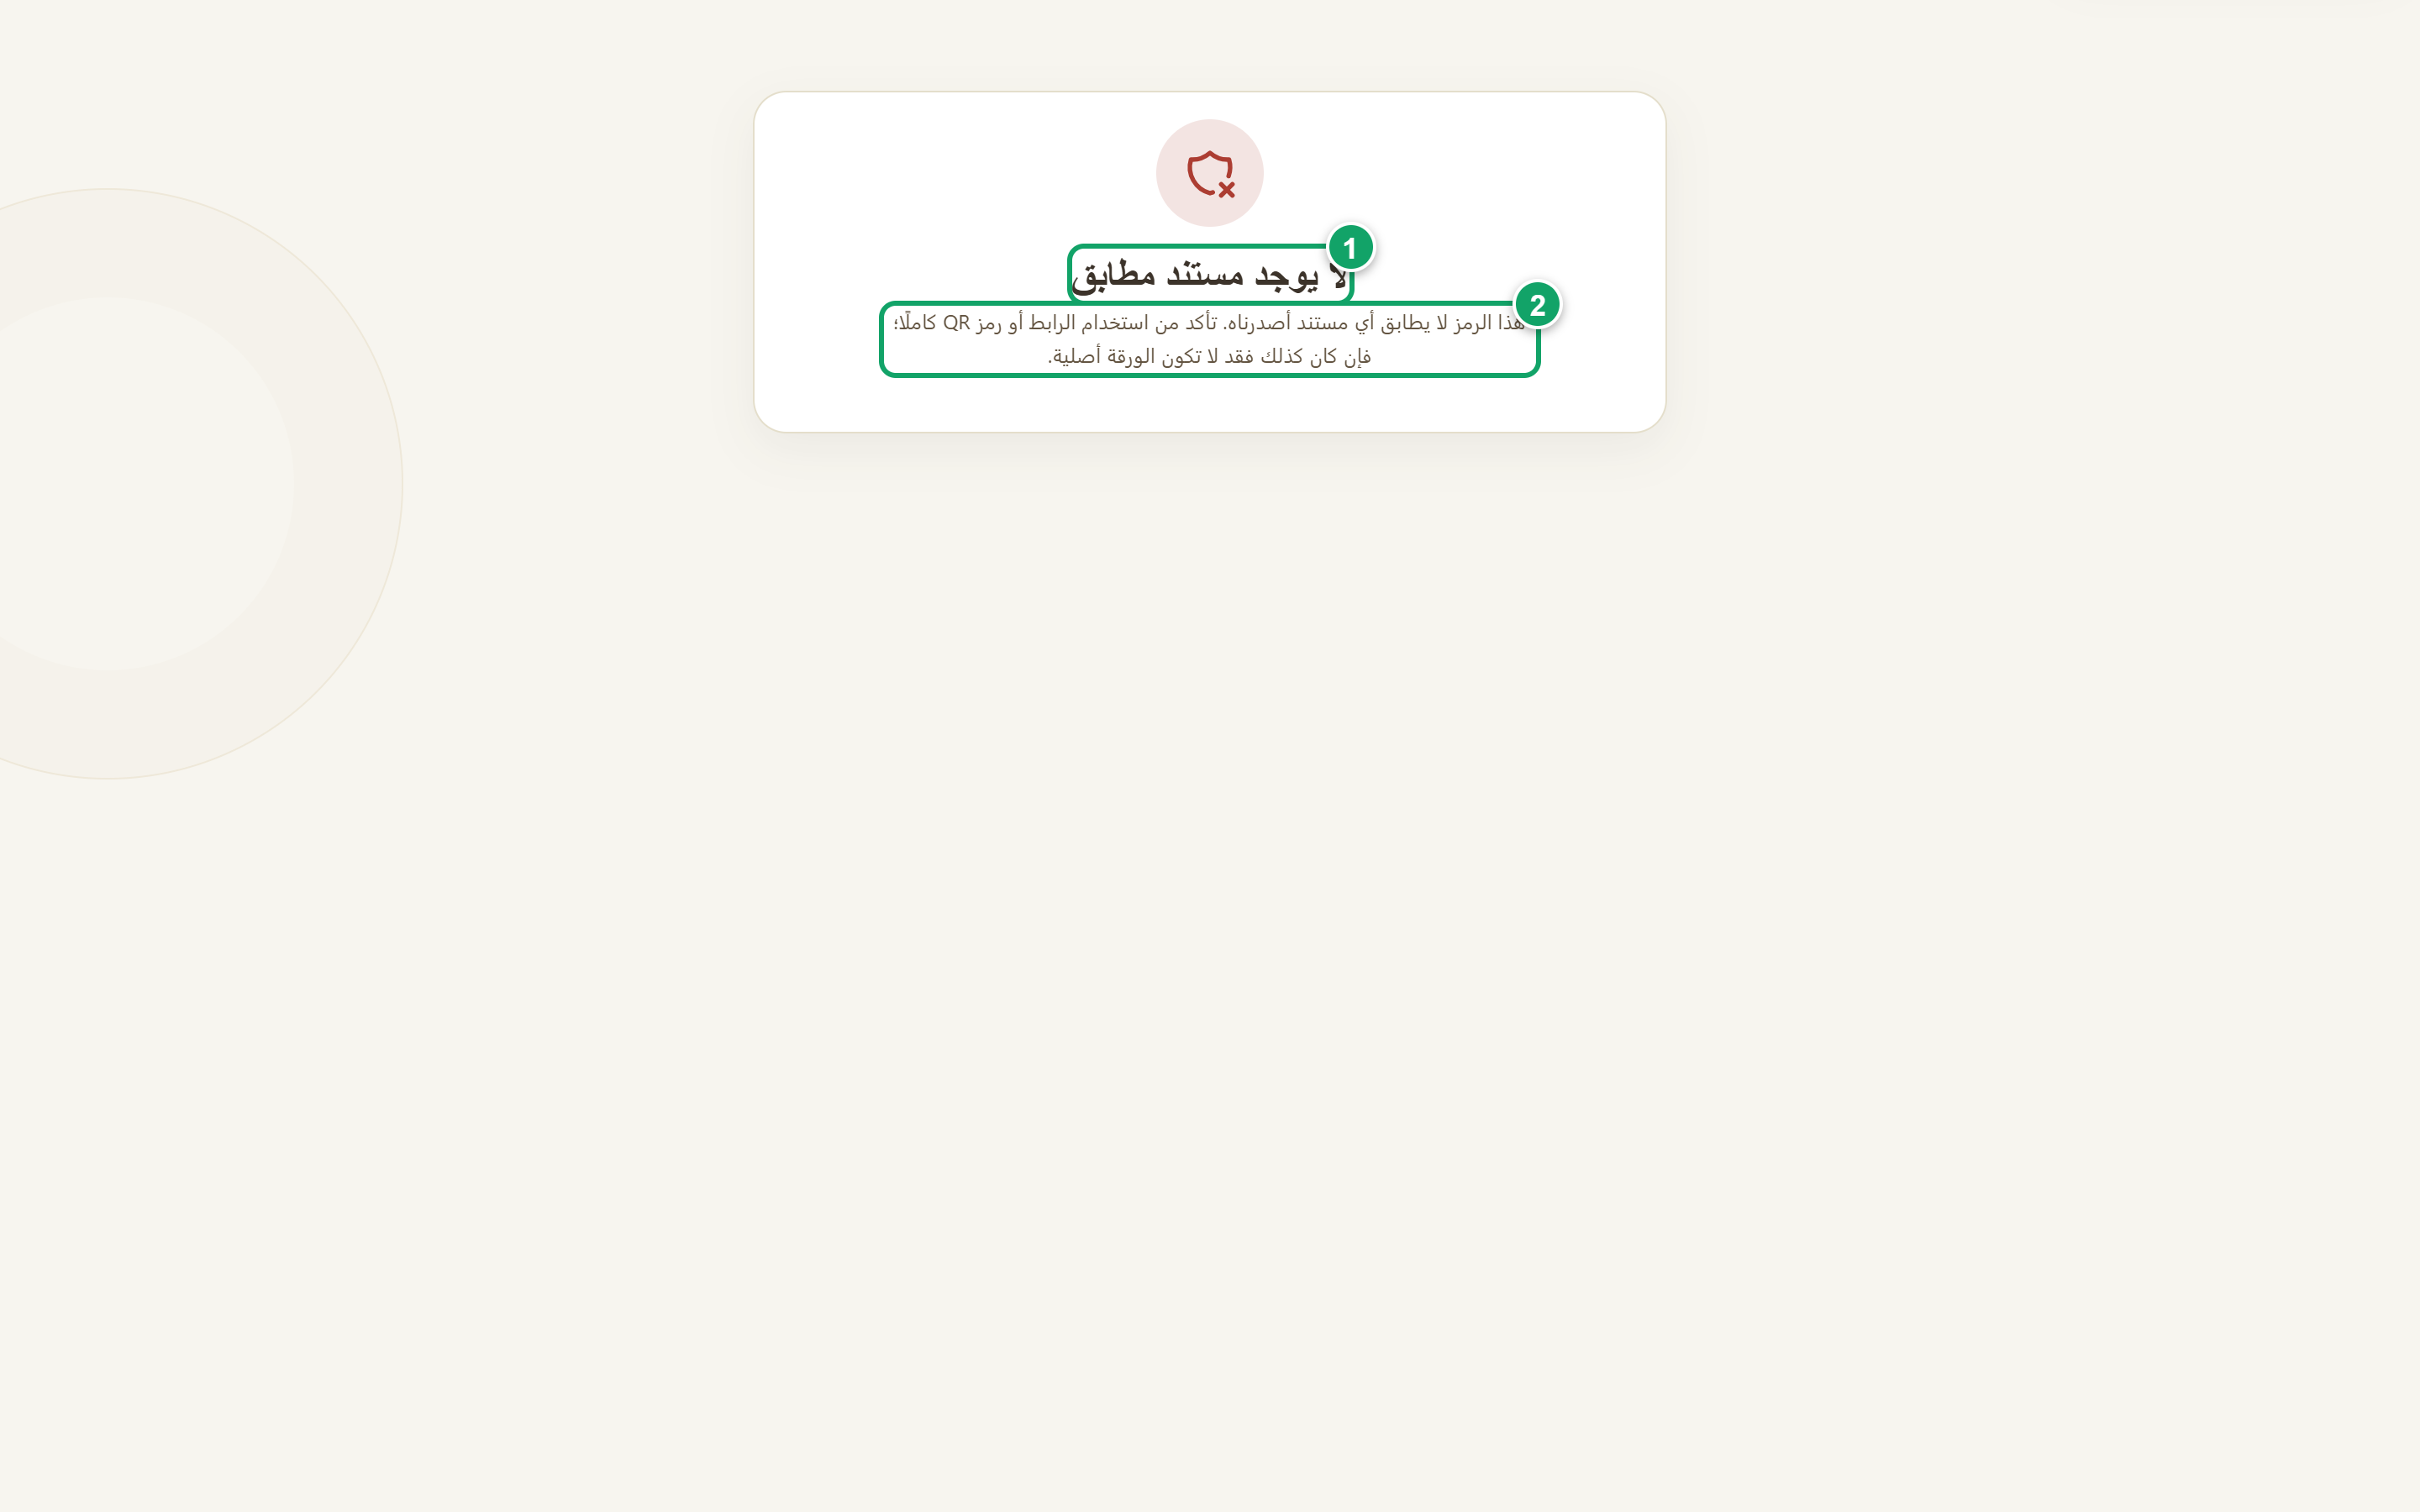
\includegraphics[width=0.95\linewidth,height=0.72\textheight,keepaspectratio]{figures/screens/ch06-print-verify-ar.png}
\caption{صفحة التحقق عند استخدام رمز غير صحيح}
\label{fig:builder-print-verify-screen}
\shotnote{تعرض الصورة صفحة التحقق العامة بعد فتحها برمز تجريبي لا يطابق أي مستند، لأن التقاطها برمز حقيقي يتطلب طباعة مستند فعلي. وهي النتيجة التي يراها من يحمل ورقة مزورة أو رابطاً منقوصاً، وتظهر دون تسجيل دخول. ① «لا يوجد مستند مطابق»: نتيجة الفحص. ② نص الإرشاد: يطلب التأكد من استخدام الرابط أو الرمز كاملاً قبل الحكم على الورقة.}
\end{figure}

\begin{table}[H]
\centering
\caption{ما تعرضه صفحة التحقق}
\label{tab:builder-print-verify-results}
\begin{tabularx}{\linewidth}{R{3.6cm} Y}
\rcHeaderRow
\thh{النتيجة} & \thh{معناها}\\
«الرمز موثّق» & صدر الرمز عن المؤسسة لهذا المستند. وتظهر «بيانات المستند»: «المستند» و«الجهة المُصدِرة» و«تاريخ الإصدار» و«إصدار القالب» و«بصمة الملف».\\
«المستند كما صدر» & نص المستند كما طُبع. وتظهر التواقيع مواضع تذكر اسم الموقّع، ولا يظهر رمز QR.\\
«تحقّق من ملف وصلك» & تختار ملف PDF أو Word وصلك، فيخبرك هل هو الملف نفسه الذي صدر. ويبقى الملف على جهازك.\\
«لا يوجد مستند مطابق» & الرمز لا يطابق أي مستند صادر، فتأكد من استخدام الرابط أو الرمز كاملاً، وإلا فقد لا تكون الورقة أصلية.\\
«تعذّر التحقق من هذا المستند الآن» & مشكلة مؤقتة لا تعني أن المستند غير أصلي، فأعد المحاولة بعد قليل.\\
\end{tabularx}
\end{table}

\begin{rcwarn}[قارن الورقة بالمستند المعروض]
إذا اختلف اسم أو رقم أو تاريخ أو مبلغ بين الورقة والمستند المعروض، فقد عُدّلت الورقة بعد إصدارها. وإذا طُبع المستند مع مستندات أخرى في ملف واحد بالطباعة الجماعية، فلا يمكن التحقق من ملفه، بل تقارن المحتوى فقط.
\end{rcwarn}

\begin{figure}[H]
\centering
\begin{tikzpicture}[node distance=0.5cm]
\node[stepBox] (a) {\RL{تفعيل رمز التحقق في المخرجات}};
\node[stepBox,below=of a] (b) {\RL{طباعة المستند برمز QR}};
\node[stepBox,below=of b] (c) {\RL{مسح الرمز}};
\node[stepBox,below=of c] (d) {\RL{مقارنة الورقة بالمستند كما صدر}};
\draw[flowsTo] (a) -- (b);
\draw[flowsTo] (b) -- (c);
\draw[flowsTo] (c) -- (d);
\end{tikzpicture}
\rclegend
\caption{من الطباعة إلى التحقق}
\label{fig:builder-print-verify-flow}
\shotnote{يبيّن المخطط أن التحقق يبدأ من قرار يتخذه مصمم القالب، فلا يحمل المستند رمزاً إذا لم يفعّله. وتنتهي الخطوات بالمقارنة لأن الصفحة تثبت ما صدر، ويبقى على القارئ أن يتأكد من أن الورقة تطابقه.}
\end{figure}

\subsection{خطوات العمل والتحقق}
\begin{enumerate}
\item فعّل «رمز QR يفتح صفحة تحقق» في «المخرجات»، وضع عنصر «رمز QR» في القالب أو في الترويسة.
\item انشر القالب، واطبع مستنداً تجريبياً من سجل.
\item امسح الرمز بهاتفك، وتأكد من ظهور «الرمز موثّق».
\item قارن «المستند كما صدر» بالورقة، وجرّب «تحقّق من ملف وصلك» بملف PDF الذي نزّلته.
\end{enumerate}

\textbf{تحقق ومعالجة المشكلة:} يجب أن تفتح الصفحة دون تسجيل دخول، وأن تطابق بياناتها الورقة. وإذا لم يُطبع الرمز على المستند، فالتحقق متوقف في هذا القالب، ففعّل «رمز QR يفتح صفحة تحقق» من «المخرجات». وإذا ظهر عند الطباعة «هذا المستند أكبر من أن يُتحقَّق منه برمز QR»، فأوقف التحقق في القالب أو اطبع صفوفاً أقل.

\clearpage
\section{الهويات والترويسات}
\label{sec:builder-feature-identities}

الهوية هي شعار المؤسسة واسمها وألوانها وبياناتها الرسمية، مثل السجل التجاري والعنوان. أما الترويسة فرأس الصفحة وتذييلها اللذان يظهران في المستندات المطبوعة. وتحفظهما هذه الصفحة في مكان واحد، فتستخدمهما قوالب الطباعة والمراسلات الرسمية معاً، وأي تغيير هنا يظهر فيها كلها في الطباعة التالية.

\textbf{المسار ومن يستخدمه:} «ادوات البناء» ← «الأساسية» ← «الهويات والترويسات». يستخدمها من يدير مظهر مستندات المؤسسة.

\begin{rcnote}[مثال: شركة الأفق]
يرفع مسؤول النظام شعار الأفق ويضيف بياناتها الرسمية إلى الهوية الافتراضية، ثم ينشئ ترويسة يظهر رأسها في الصفحة الأولى فقط، فتطبع ورقة الزيارة بشعار الشركة دون إعادة تصميمه في كل قالب. ويرفع الشعار في ③ ويحفظ من ④، ثم ينشئ الترويسة من ②.
\end{rcnote}

\begin{figure}[H]
\centering
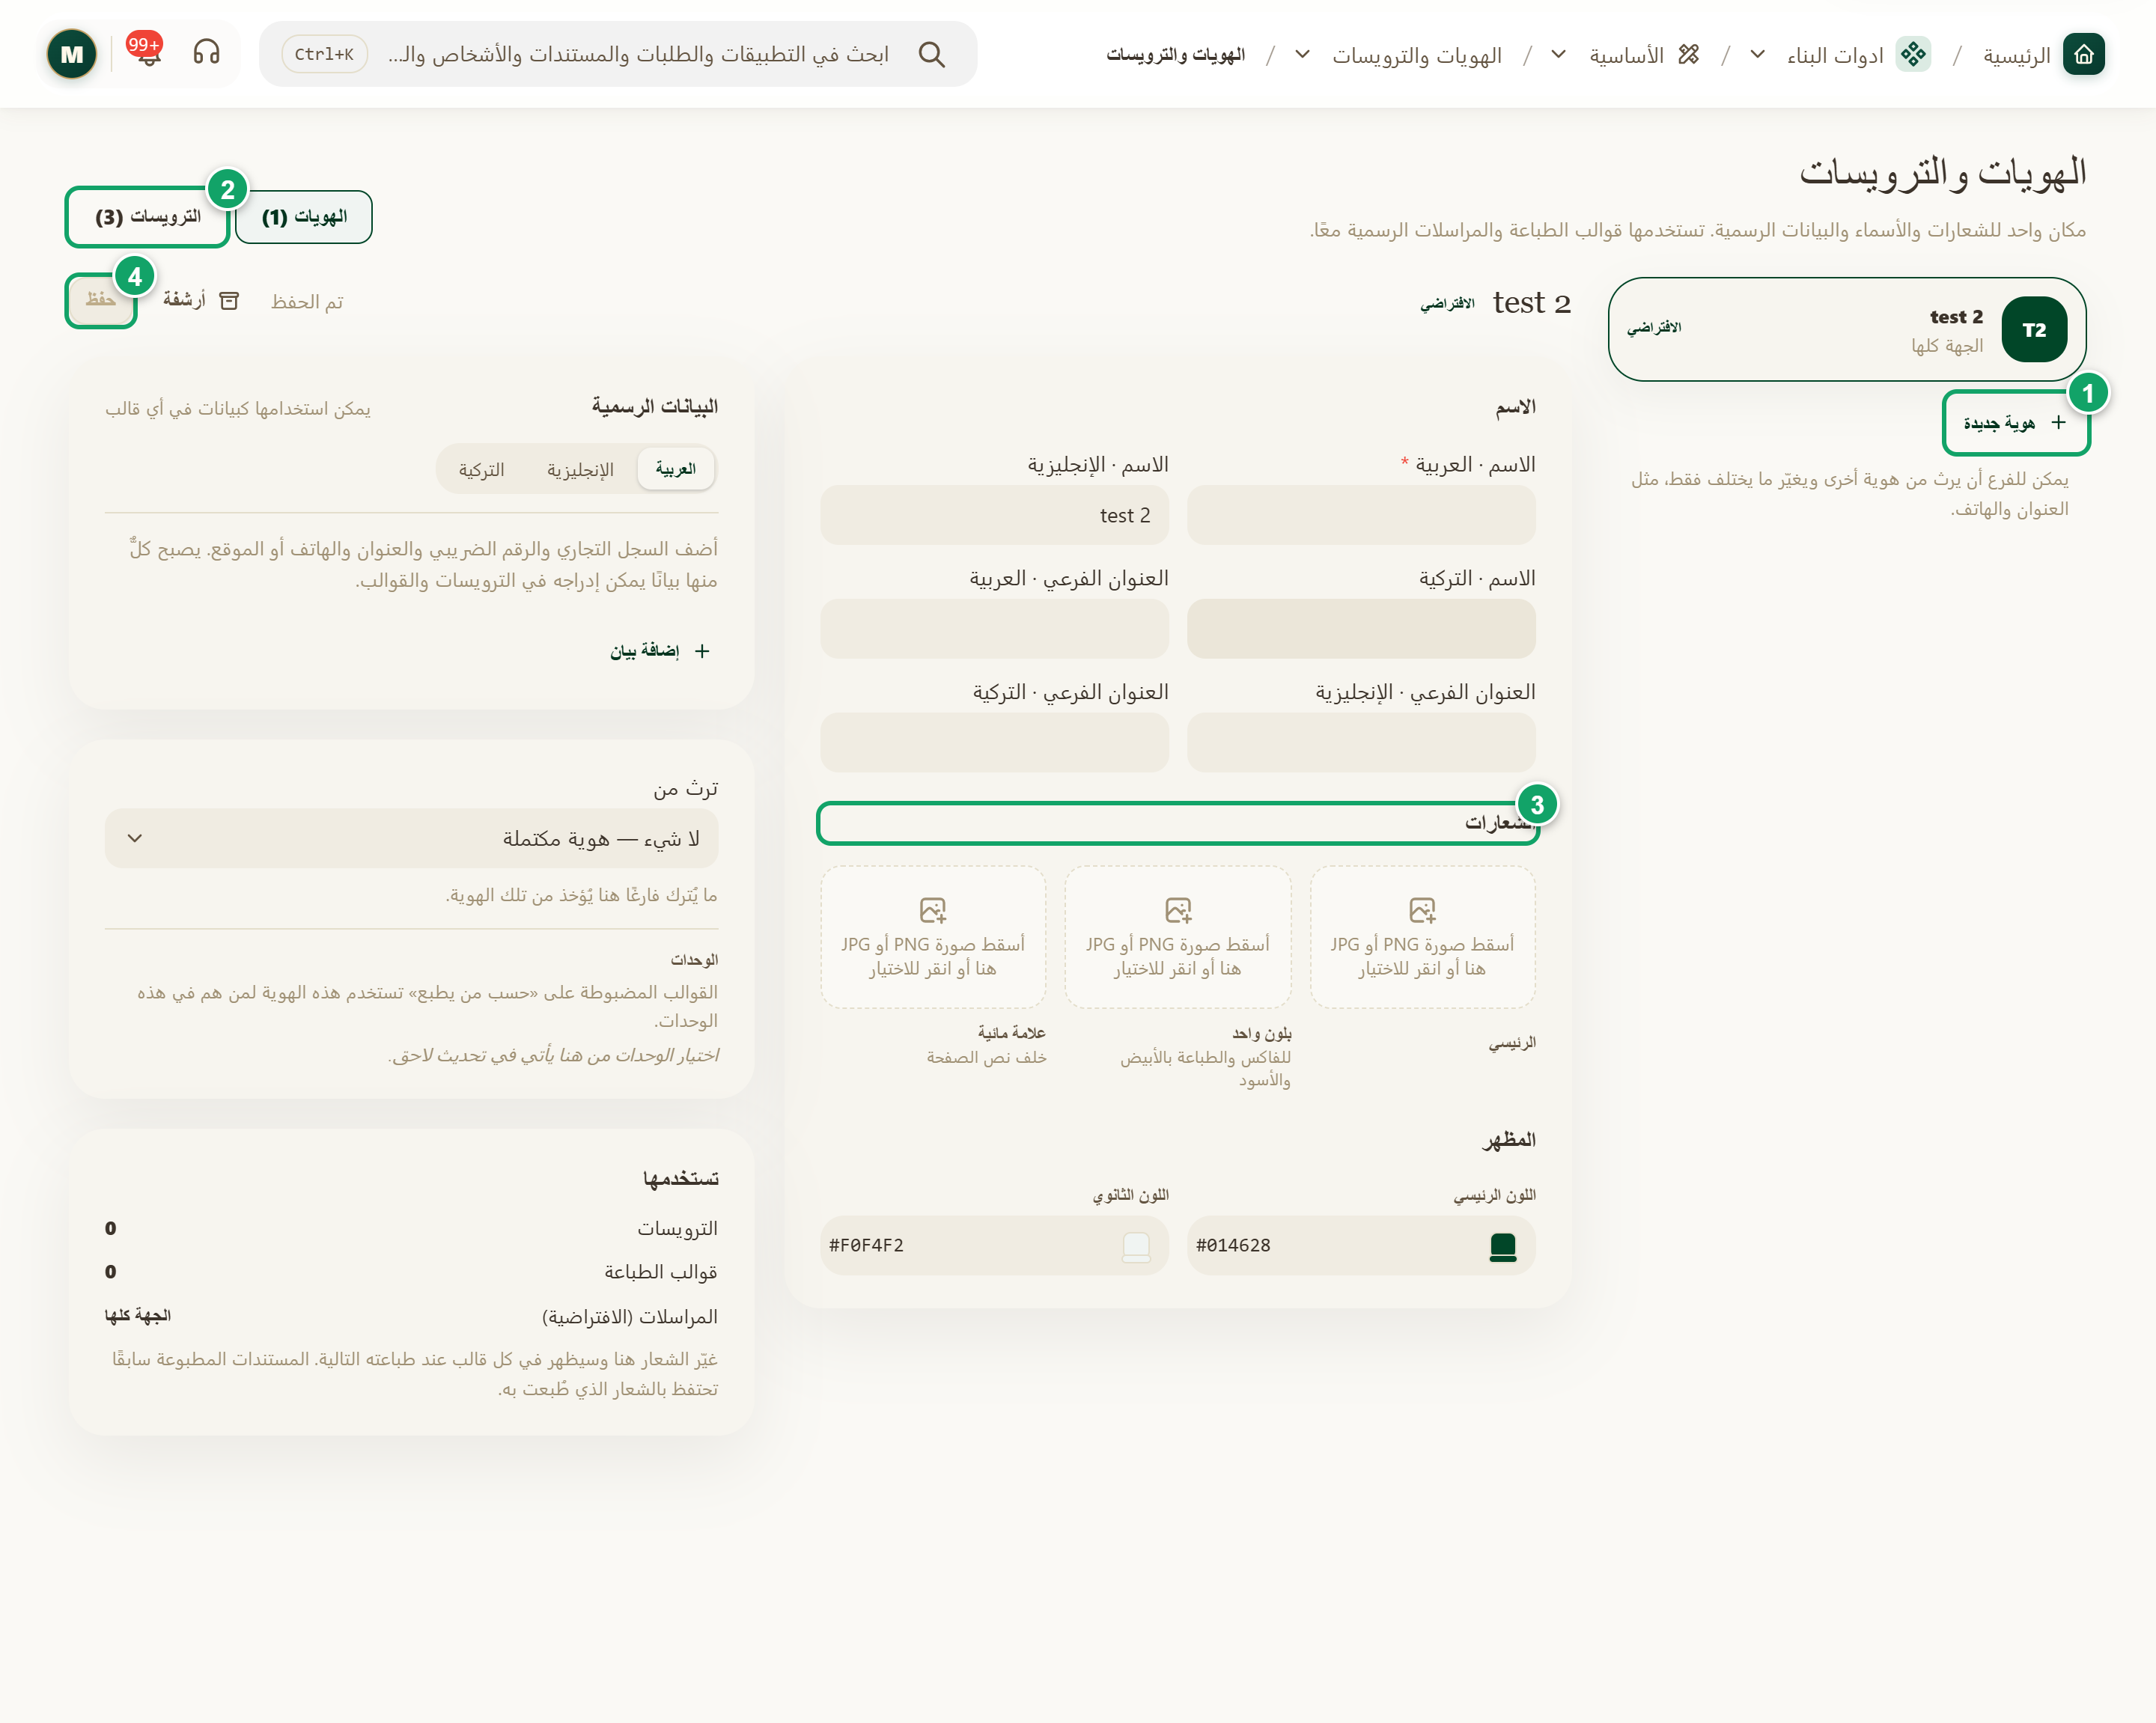
\includegraphics[width=0.95\linewidth,height=0.72\textheight,keepaspectratio]{figures/screens/ch06-identities-ar.png}
\caption{صفحة «الهويات والترويسات»}
\label{fig:builder-identities-screen}
\shotnote{تعرض الصفحة الهوية الافتراضية للمؤسسة وحقولها، وهي هنا هوية مؤسسة الاختبار. ① «هوية جديدة»: تنشئ هوية أخرى، مثل هوية فرع. ② «الترويسات»: تبويب الترويسات المشتركة. ③ «الشعارات»: الشعار الرئيسي وبلون واحد والعلامة المائية. ④ «حفظ»: يحفظ تعديل الهوية.}
\end{figure}


\begin{table}[H]
\centering
\caption{ما الذي تجده هنا؟}
\label{tab:builder-identities-data}
\begin{tabularx}{\linewidth}{R{3.6cm} Y}
\rcHeaderRow
\thh{الجزء} & \thh{المحتوى والإجراء}\\
الهويات & لكل هوية «الاسم» و«العنوان الفرعي» بكل لغة، و«الشعارات» (الرئيسي، بلون واحد، علامة مائية)، و«المظهر» بلونين، و«البيانات الرسمية».\\
ترث من & تجعل الهوية تأخذ ما لم تحدده من هوية أخرى، مثل هوية فرع ترث من هوية المؤسسة.\\
تستخدمها & تبيّن الترويسات وقوالب الطباعة والمراسلات التي تعتمد على الهوية.\\
الترويسات & قائمة الترويسات المشتركة، ولكل ترويسة عدد القوالب التي تستخدمها، ومنها «تعديل» و«نسخ» و«اجعله الافتراضي» و«أرشفة».\\
\end{tabularx}
\end{table}

\begin{figure}[H]
\centering
\begin{tikzpicture}[node distance=0.5cm]
\node[entity] (id) {\RL{الهوية}};
\node[entityOpt,below=0.7cm of id] (lh) {\RL{الترويسة}};
\node[entityOpt,below right=0.7cm and 0.3cm of lh] (print) {\RL{قوالب الطباعة}};
\node[entityOpt,below left=0.7cm and 0.3cm of lh] (corr) {\RL{المراسلات الرسمية}};
\draw[dependsOnOpt] (id) -- (lh);
\draw[dependsOnOpt] (lh.south) -- ++(0,-0.3) -| (print.north);
\draw[dependsOnOpt] (lh.south) -- ++(0,-0.3) -| (corr.north);
\end{tikzpicture}
\rclegend
\caption{من الهوية إلى المستند المطبوع}
\label{fig:builder-identities-model}
\shotnote{يوضّح الشكل أن الهوية تغذّي الترويسة، وأن الترويسة مشتركة بين قوالب الطباعة والمراسلات الرسمية. لذلك عدّل الشعار أو البيانات الرسمية في الهوية مرة واحدة، فيظهر التعديل في كل مستند يُطبع بعد ذلك؛ وراجع «تستخدمها» قبل أي تغيير.}
\end{figure}

\subsection{خطوات العمل والتحقق}
\begin{enumerate}
\item افتح «الهويات والترويسات»، واختر الهوية الافتراضية «الجهة كلها» أو أنشئ «هوية جديدة».
\item اكتب الاسم بكل لغة، وارفع الشعارات بصيغة PNG أو JPG، وأضف البيانات الرسمية، ثم اضغط «حفظ».
\item افتح «الترويسات»، وأنشئ «ترويسة جديدة»، واختر عناصرها ومكان ظهورها.
\end{enumerate}

\textbf{تحقق ومعالجة المشكلة:} اطبع مستنداً تجريبياً من قالب يستخدم الترويسة، فيجب أن يظهر الشعار والبيانات الجديدة. وإذا لم تستطع أرشفة هوية، فاجعل هوية أخرى هي الافتراضية أولاً، لأن الهوية الافتراضية لا تُؤرشف.

\clearpage
\section{محرر الترويسة}
\label{sec:builder-feature-letterheads}

الترويسة رأس صفحة وتذييل تصممهما مرة واحدة، فتستخدمهما قوالب الطباعة والمراسلات الرسمية. ويعرض محرر الترويسة ورقة فيها منطقتان: «الرأس» في أعلاها و«التذييل» في أسفلها، وبينهما مكان محتوى كل قالب. وتضيف إلى المنطقتين نصاً تكتبه بنفسك، أو بيانات من الهوية والمستند تتغير مع كل طباعة، مثل اسم الجهة وتاريخ الطباعة ورقم الصفحة. وأي تغيير تحفظه هنا يظهر في كل قالب يستخدم الترويسة وفي الخطابات الرسمية أيضاً.

\textbf{المسار ومن يستخدمه:} «ادوات البناء» ← «الأساسية» ← «الهويات والترويسات» ← «الترويسات» ← «ترويسة جديدة» أو «تعديل». يستخدمه من يدير مظهر مستندات المؤسسة.

\begin{rcnote}[مثال: شركة الأفق]
ينشئ مسؤول النظام ترويسة باسم «ترويسة الأفق»، ويضع في رأسها الشعار والاسم، وفي تذييلها عنوان المقر الرئيسي في دمشق ورقم الصفحة. ثم يجعل الرأس يظهر في الصفحة الأولى فقط والتذييل في كل صفحة، ويضغط «حفظ». فيكتب الاسم في ①، ويدرج الشعار من ② ورقم الصفحة من ③، ويحدد الصفحات بجانب ④، ثم يحفظ بـ ⑤.
\end{rcnote}

\begin{figure}[H]
\centering
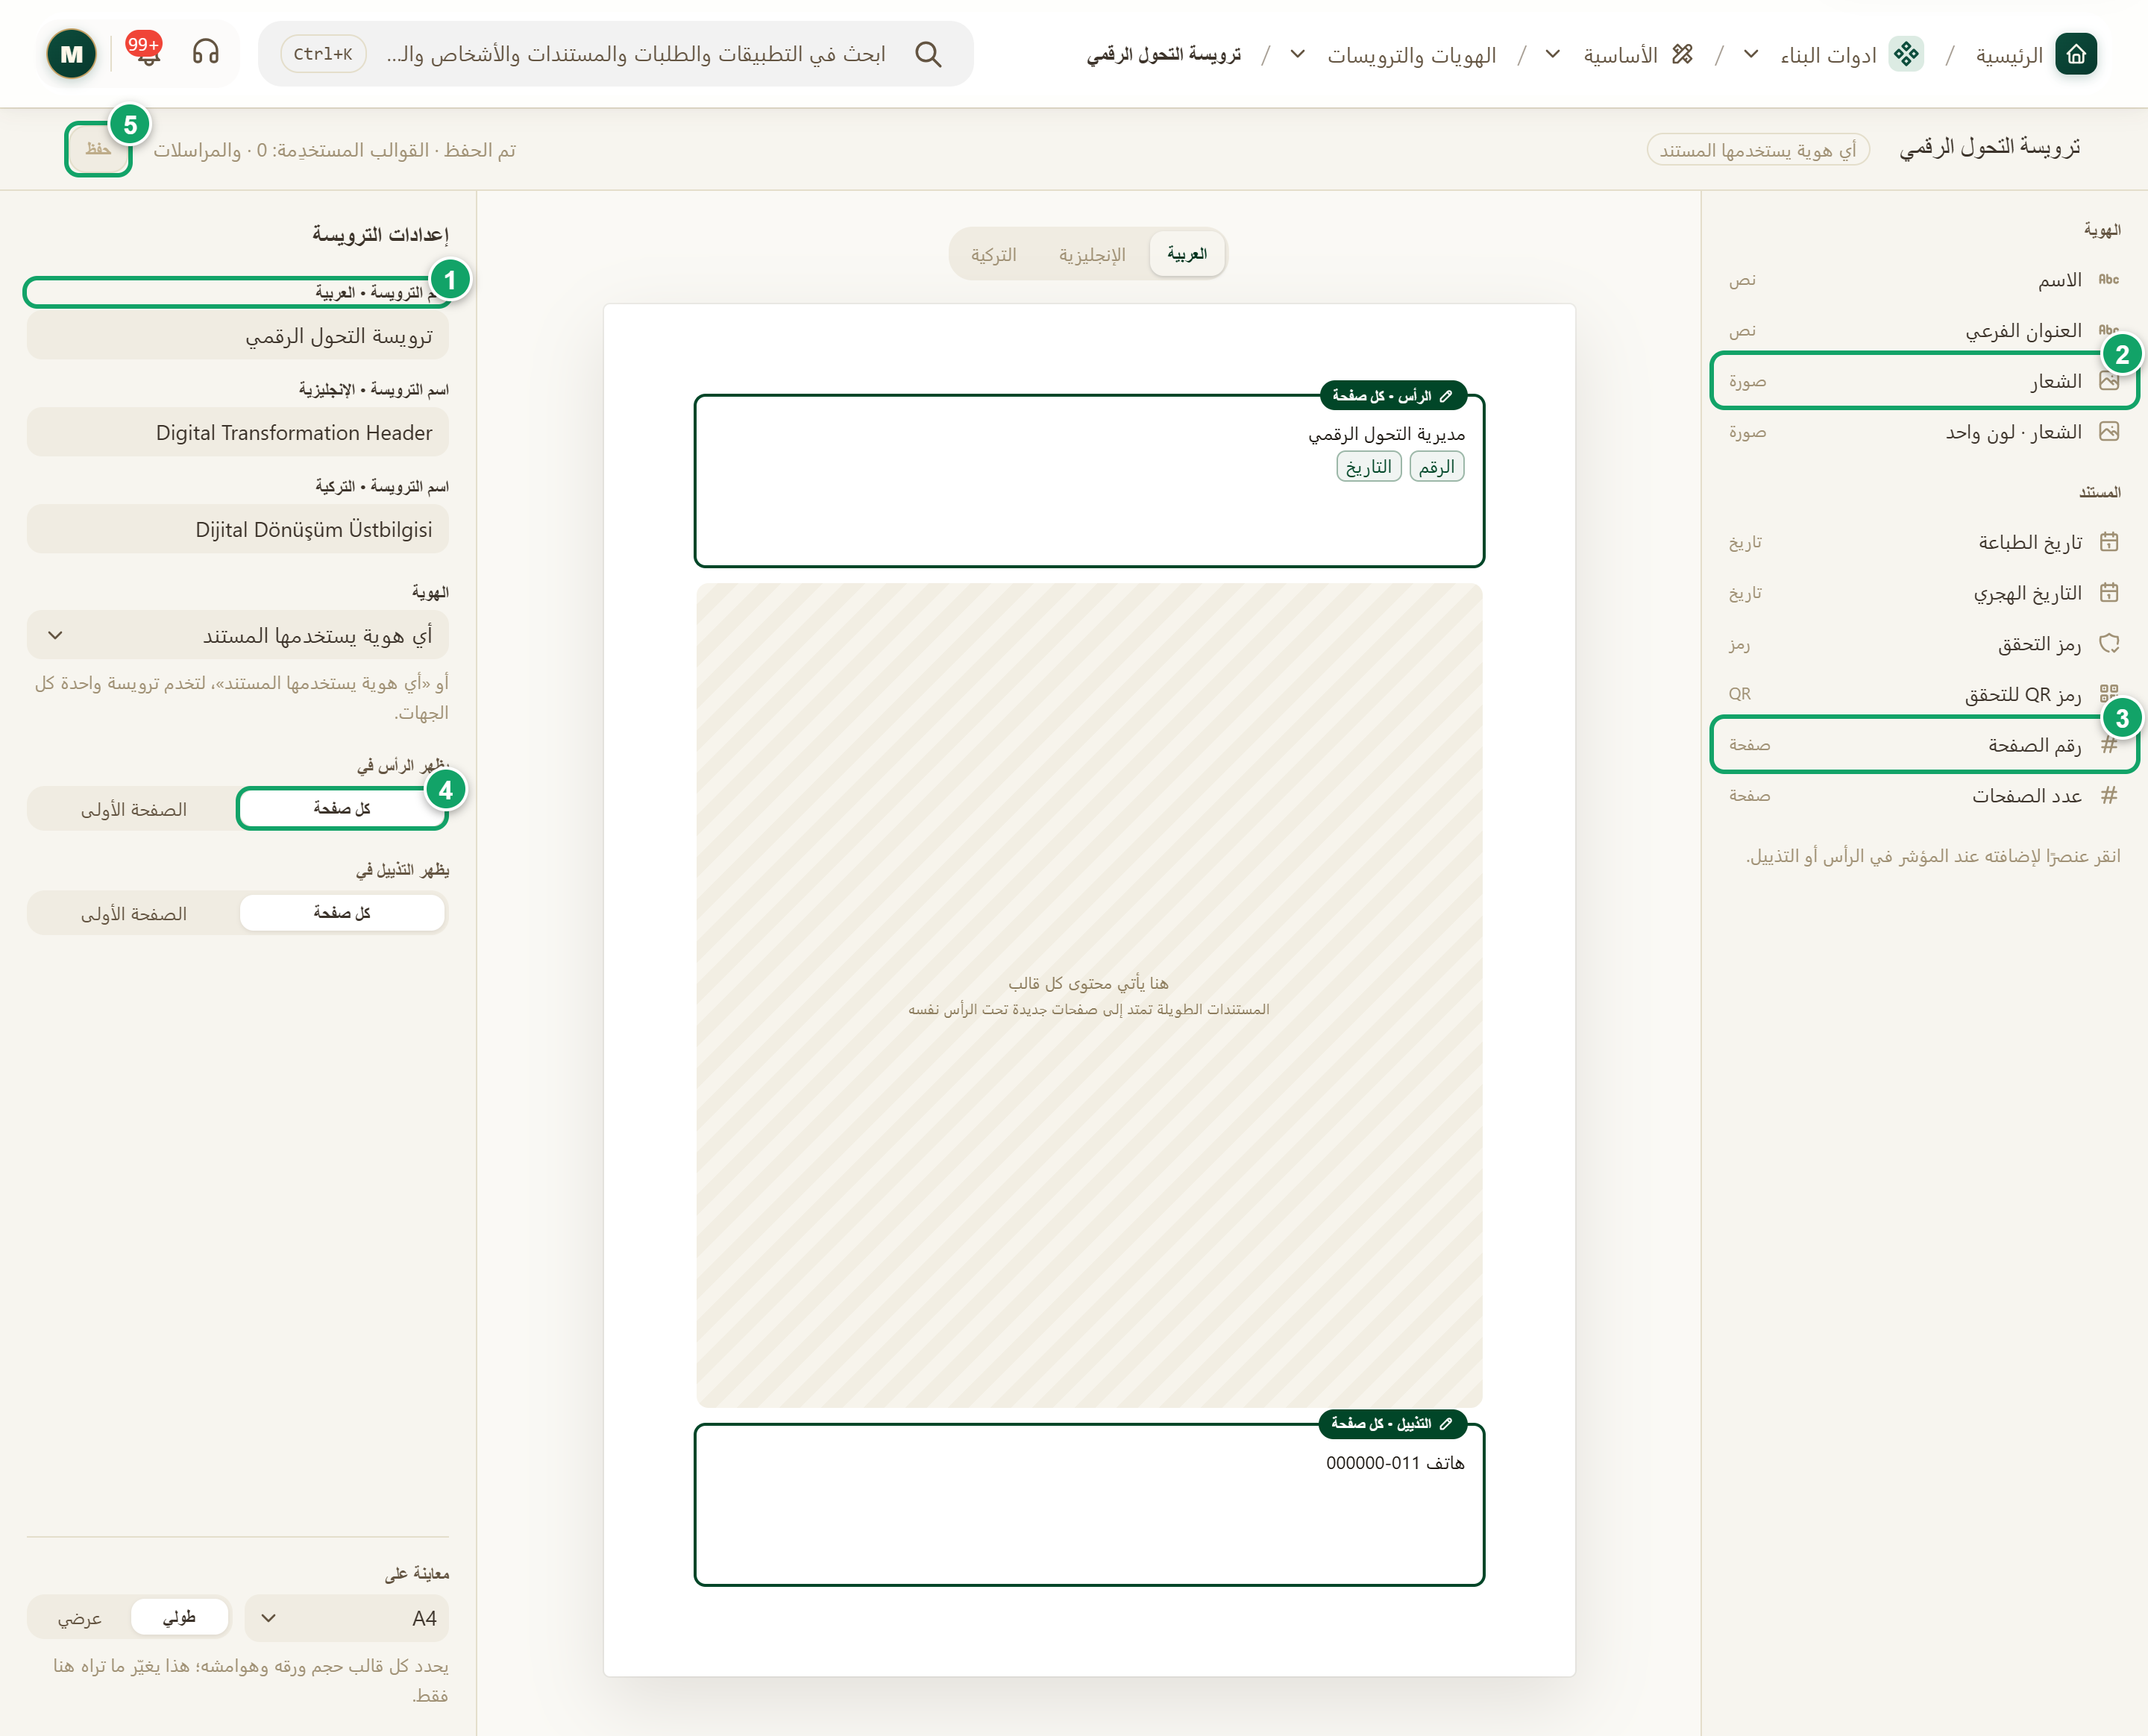
\includegraphics[width=0.95\linewidth,height=0.72\textheight,keepaspectratio]{figures/screens/ch06-letterheads-ar.png}
\caption{محرر الترويسة لترويسة موجودة}
\label{fig:builder-letterheads-screen}
\shotnote{تعرض الصورة ترويسة اختبارية في test2 مفتوحة في المحرر على اللغة العربية، وفي رأسها نص وعنصران من البيانات، وفي تذييلها رقم هاتف. ويبيّن السطر بجانب زر الحفظ عدد القوالب التي تستخدم الترويسة، فتعرف أثر أي تغيير قبل حفظه. ① «اسم الترويسة · العربية»: الاسم الذي يظهر عند اختيار الترويسة في القوالب. ② «الشعار»: يُدرَج من بيانات الهوية في موضع المؤشر. ③ «رقم الصفحة»: من بيانات المستند. ④ «كل صفحة»: الصفحات التي يظهر فيها الرأس. ⑤ «حفظ»: يحفظ الترويسة لكل من يستخدمها.}
\end{figure}

\begin{table}[H]
\centering
\caption{قائمة «البيانات» في المحرر}
\label{tab:builder-letterheads-data}
\begin{tabularx}{\linewidth}{R{3.6cm} Y}
\rcHeaderRow
\thh{المجموعة} & \thh{العناصر}\\
«الهوية» & «الاسم» و«العنوان الفرعي» و«الشعار» و«الشعار · لون واحد»، وكل بيان أضفته في «البيانات الرسمية» للهوية، مثل الرقم الضريبي.\\
«المستند» & «تاريخ الطباعة» و«التاريخ الهجري» و«رمز التحقق» و«رمز QR للتحقق» و«رقم الصفحة» و«عدد الصفحات».\\
\end{tabularx}
\end{table}

تضيف العنصر بالضغط عليه، فيُدرج في موضع المؤشر داخل الرأس أو التذييل.

\begin{table}[H]
\centering
\caption{«إعدادات الترويسة»}
\label{tab:builder-letterheads-settings}
\begin{tabularx}{\linewidth}{R{3.6cm} Y}
\rcHeaderRow
\thh{الإعداد} & \thh{ما يحدده}\\
«اسم الترويسة» & اسم يظهر عند اختيار الترويسة في القوالب، ويُكتب بكل لغة من لغات المؤسسة.\\
«الهوية» & هوية بعينها، أو «أي هوية يستخدمها المستند» لتخدم ترويسة واحدة كل الهويات.\\
«يظهر الرأس في» و«يظهر التذييل في» & «كل صفحة» أو «الصفحة الأولى».\\
«معاينة على» & «طولي» أو «عرضي»، وتغيّر ما تراه في المحرر فقط، لأن كل قالب يحدد ورقه وهوامشه بنفسه.\\
«لغة الترويسة» & تبويبات تظهر عندما يكون للمؤسسة أكثر من لغة، فتصمم نسخة الترويسة لكل لغة.\\
\end{tabularx}
\end{table}

\begin{figure}[H]
\centering
\begin{tikzpicture}[node distance=0.5cm]
\node[stepBox] (a) {\RL{ترويسة جديدة}};
\node[stepBox,below=of a] (b) {\RL{كتابة الرأس والتذييل}};
\node[stepBox,below=of b] (c) {\RL{إدراج بيانات الهوية والمستند}};
\node[stepBox,below=of c] (d) {\RL{ضبط الهوية والصفحات}};
\node[stepBox,below=of d] (e) {\RL{حفظ واختيارها في القوالب}};
\draw[flowsTo] (a) -- (b);
\draw[flowsTo] (b) -- (c);
\draw[flowsTo] (c) -- (d);
\draw[flowsTo] (d) -- (e);
\end{tikzpicture}
\rclegend
\caption{إعداد ترويسة مشتركة}
\label{fig:builder-letterheads-flow}
\shotnote{يبيّن المخطط أن الترويسة تُصمَّم مرة واحدة ثم تُختار في كل قالب، فلا تُعاد كتابتها في كل مستند. ويأتي إدراج بيانات الهوية بدلاً من كتابتها نصاً ثابتاً، لأن تغيير الشعار أو العنوان في الهوية يصل عندئذ إلى الترويسة تلقائياً.}
\end{figure}

\subsection{خطوات العمل والتحقق}
\begin{enumerate}
\item افتح «الهويات والترويسات»، ثم «الترويسات»، واضغط «ترويسة جديدة».
\item اكتب «اسم الترويسة»، واختر «الهوية» من «إعدادات الترويسة».
\item اضغط داخل الرأس، واكتب ما تريد، ثم أضف «الشعار» و«الاسم» من قائمة «البيانات».
\item اضغط داخل التذييل، وأضف العنوان أو بيانات التواصل و«رقم الصفحة».
\item اختر الصفحات التي يظهر فيها الرأس والتذييل، ثم اضغط «حفظ».
\end{enumerate}

\textbf{تحقق ومعالجة المشكلة:} يجب أن تتحول الحالة إلى «تم الحفظ» مع عدد القوالب التي تستخدم الترويسة، وأن تظهر الترويسة في قائمة الترويسات. فإذا ظهر «أدخل اسمًا للترويسة.»، فاكتب الاسم ثم احفظ. وإذا ظهر عند الأرشفة «ما زالت قوالب طباعة تستخدم هذه الترويسة»، فاختر ترويسة أخرى في تلك القوالب أولاً.
